\chapter[Propriedades de \texorpdfstring{$B_n$}{Bn} e o grupo de tranças puras]{Propriedades de \texorpdfstring{$B_n$}{Bn} e o grupo de tranças puras}
\label{cap-4}
\chaptermark{}
%
\hfill%
\begin{minipage}{10cm}
\begin{flushright}
\rightskip=0.5cm
\textit{``The essence of math is not to make simple things complicated, but to make complicated things simple.''}
\\[0.1cm]
\rightskip=0.5cm
--- Stan Gudder
\end{flushright}
\end{minipage}

\section{Primeiras propriedades}

    Vamos demonstrar algumas propriedades das tranças. Para evitar confusões, por vezes será usada a notação $1_n$ para indicar a identidade de $B_n$.
	
	%\begin{prop}
	%	\label{centro de B_n}
	%	Para $1\leq i\leq n-1$, $(\sigma_1\sigma_2\cdots\sigma_{n-1})^n\sigma_i = \sigma_i(\sigma_1\sigma_2\cdots\sigma_{n-1})^n$, ou seja, $(\sigma_1\sigma_2\cdots\sigma_{n-1})^n$ pertence ao centro de $B_n$.
	%\end{prop}
	
	%\begin{proof}
	
	%\end{proof}
	
	%\begin{remark}
	%	É possível mostrar que $(\sigma_1\sigma_2\cdots\sigma_{n-1})^n$ gera o centro de $B_n$. Além disso, como $l((\sigma_1\sigma_2\cdots\sigma_{n-1})^n)\neq 0 = l(1_n)$ (sendo $l$ a função definida no Lema \eqref{homomorfismo de comprimento}), então $(\sigma_1\sigma_2\cdots\sigma_{n-1})^n\neq 1_n$ e, consequentemente, o centro de $B_n$ não é trivial.
	%\end{remark}
	
	\begin{prop}
		\label{B_m subgrupo de B_n}
		Para $1\leq m\leq n$, o mapa $\psi: \underset{\sigma_i\mapsto\sigma_i}{B_m\to B_n}$ para $1\leq i\leq m-1$ é um homomorfismo injetor de $B_m$ em $B_n$ e então podemos considerar $B_m$ um subgrupo de $B_n$. 
	\end{prop}
	
	
	\begin{proof}
		Pelo Teorema \eqref{apresentacao de B_n}, temos
		
		\begin{align*}
		B_m = \langle \sigma_1, \sigma_2, \dots, \sigma_{m-1} | &\sigma_i\sigma_j = \sigma_j\sigma_i, \text{ para }|i-j|>1 \\ 
		&\sigma_i\sigma_{i+1}\sigma_i = \sigma_{i+1}\sigma_i\sigma_{i+1}, 1\leq i\leq m-2\rangle \\
		B_n = \langle \sigma_1, \sigma_2, \dots, \sigma_{m-1}, \dots, \sigma_{n-1} | \sigma_i\sigma_j = &\sigma_j\sigma_i, \text{ para }|i-j|>1 \\ 
		&\sigma_i\sigma_{i+1}\sigma_i = \sigma_{i+1}\sigma_i\sigma_{i+1}, 1\leq i\leq n-2\rangle
		\end{align*} 
		
		\par\vspace{0.3cm} Daí, como $B_n$ satisfaz as relações de $B_m$, então pelo Teorema \eqref{teorema de Dyck}, $\psi$ é homomorfismo.
		
		\par\vspace{0.3cm} Agora, suponha que existe $\beta\in B_n$ tal que $\psi(\beta) = 1_n$, ou seja, existe uma trança $\beta$ de $m$ cordas que, quando adicionamos $n-m$ cordas retas, se torna a trança trivial em $B_n$. Mas então devemos ter $\beta = 1_m$, logo $\psi$ é injetora.
		
	\end{proof}
	
	\begin{remark}
		\begin{enumerate}
			\item Como consequência da Proposição \eqref{B_m subgrupo de B_n}, se $\beta\in B_m$ é não trivial, então $\beta\in B_n$, $n\geq m$, também é não trivial (sendo $\beta\in B_n$ a trança $\beta$ de $m$ cordas adicionada de $n-m$ cordas retas).
			\item Outra observação interessante é o fato de que, Em particular, $B_m\cong B_n$ se, e só se, $m=n$.
		\end{enumerate}
	\end{remark}
	
	\begin{prop}
		\label{geradores de B_n tem ordem infinita}
		$B_n$ é \textbf{livre de torção}, i.e., todo gerador de $B_n$ tem ordem infinita. Equivalentemente, $\sigma_i^k \neq 1, \forall k\in\mathbb{Z}^{\ast}$.
	\end{prop}
	
	\begin{proof}
		Vamos demonstrar a Proposição \eqref{geradores de B_n tem ordem infinita} por indução em $i$, o índice dos geradores.	Como $B_2 = \langle \sigma_1 | - \rangle$, então $|\sigma_1| = \infty$. Logo, em $B_n$, $|\sigma_1| = \infty$. Suponha, então, que $\sigma_2\in B_n$ tem ordem finita. Logo, por definição, $\exists l\in\mathbb{Z}$ tal que $\sigma_2^l = 1_n$. Daí, 
		
		\begin{equation*}
		(\sigma_1\sigma_2\sigma_1)\sigma_2^l(\sigma_1\sigma_2\sigma_1)^{-1} = 1_n
		\end{equation*}
		
		\par\vspace{0.3cm} Note que como $\sigma_i\sigma_{i+1}\sigma_i = \sigma_{i+1}\sigma_i\sigma_{i+1}$, então $\sigma_i\sigma_{i+1}\sigma_i^{-1} = \sigma_{i+1}^{-1}\sigma_i\sigma_{i+1}$ e, consequentemente, $\sigma_i\sigma_{i+1}^l\sigma_i^{-1} = \sigma_{i+1}^{-1}\sigma_i^l\sigma_{i+1}$. Substituindo na equação acima, temos
		
		\begin{align*}
		1_n &= \sigma_1\sigma_2\sigma_1\sigma_2^l\sigma_1^{-1}\sigma_2^{-1}\sigma_1^{-1} \\
		&= \sigma_1\sigma_2\sigma_2^{-1}\sigma_1^l\sigma_2\sigma_2^{-1}\sigma_1^{-1} \\
		&= \sigma_1^l
		\end{align*}
		
		\par\vspace{0.3cm} o que é absurdo, logo $|\sigma_2| = \infty$.
		
		\par\vspace{0.3cm} Então, suponha indutivamente que $|\sigma_j| = \infty, 1\leq j\leq i-1$. Suponha que $|\sigma_i| = l, l\in\mathbb{Z}$. Então, 
		
		\begin{align*}
		1_n &= \sigma_{i-1}\sigma_i\sigma_{i-1}\sigma_i^l\sigma_{i-1}^{-1}\sigma_i^{-1}\sigma_{i-1}^{-1} \\
		&= \sigma_{i-1}\sigma_i\sigma_i^{-1}\sigma_{i-1}^l\sigma_i\sigma_i^{-1}\sigma_{i-1}^{-1} \\
		&= \sigma_{i-1}^l
		\end{align*}
		
		\par\vspace{0.3cm} o que é absurdo também. Então, por indução, $|\sigma_i| = \infty, i\geq 1$. 
	\end{proof}
	
	\begin{remark}
		Como todo elemento não trivial de $B_n$ tem ordem infinita, é possível mostrar que para toda trança $\beta$ não trivial de $B_n$, $\beta^k\neq 1_n$ se $k\neq 0$.
	\end{remark}
	
	\begin{prop}
		\label{sigma1 e alfa geram B_n}
		O grupo $B_n$, $n\geq 1$, é gerado pelos elementos $\sigma_1$ e $\alpha = \sigma_1\sigma_2\cdots\sigma_{n-1}$.
	\end{prop}
	
	\begin{proof}
		Queremos obtes os $\sigma_i$, $i\geq 2$, em termos de $\sigma_1$ e $\alpha$. Primeiro, vamos mostrar que 
		
		\begin{equation}
		\label{conjugacao}
		\sigma_{i+1} = \alpha\sigma_i\alpha^{-1}
		\end{equation} 
		
		\par\vspace{0.3cm} Para isso, note que 
		
		\begin{align*}
		\alpha\sigma_i &= \sigma_1\sigma_2\cdots\sigma_{i-1}\sigma_i\sigma_{i+1}\sigma_{i+2}\cdots\sigma_{n-1}\sigma_i \\ 
		&=\sigma_1\sigma_2\cdots\sigma_{i-1}(\sigma_{i}\sigma_{i+1}\sigma_i)\sigma_{i+2}\cdots\sigma_{n-1}  \\
		&= \sigma_1\sigma_2\cdots\sigma_{i-1}(\sigma_{i+1}\sigma_i\sigma_{i+1})\sigma_{i+2}\cdots\sigma_{n-1} \\
		&= \sigma_{i+1}\sigma_1\sigma_2\cdots\sigma_{i-1}\sigma_i\sigma_{i+1}\cdots\sigma_{n-1} \\
		&= \sigma_{i+1}\alpha
		\end{align*}
		
		\par\vspace{0.3cm} em que usamos as duas relações do Teorema \eqref{apresentacao de B_n}. Mas $\alpha\sigma_i = \sigma_{i+1}\alpha$ é equivalente à equação \eqref{conjugacao}, como queríamos demonstrar.
		
		\par\vspace{0.3cm} Agora, vamos mostrar, por indução, que $\sigma_i = \alpha^{i-1}\sigma_1\alpha^{1-i}$. 
		
		\par\vspace{0.3cm} Para $i=1$, temos $\sigma_1 = \alpha^0\sigma_1\alpha^0 = \sigma_1$. Suponha que $\sigma_{i-1} = \alpha^{(i-1)-1}\sigma_1\alpha^{1-(i-1)}$. Daí, temos
		
		\begin{align*}
		\alpha^{i-1}\sigma_1\alpha^{1-i} &= \alpha\Big( \alpha^{(i-1)-1}\sigma_1\alpha^{1- (i-1)} \Big) \alpha^{-1} \\
		&= \alpha\sigma_{i-1}\alpha^{-1} \\
		&= \sigma_i
		\end{align*}
		
		\par\vspace{0.3cm} em que usamos a equação \eqref{conjugacao} na última igualdade. 
		
		\par\vspace{0.3cm} Ora! Então, como $\sigma_i = \alpha^{i-1}\sigma_1\alpha^{1-i}$, podemos representar todo gerador de $B_n$ em termos de $\sigma_1$ e $\alpha$. Consequentemente, $\sigma_1$ e $\alpha$ geram $B_n$.
		
	\end{proof}
	
	\begin{deff}
		\label{def P_n}
		O núcleo do homomorfismo $\pi$ definido no Lema \eqref{B_n iso S_n} é chamado grupo de tranças puras e denotado por $P_n$. Uma trança geométrica de $n$ cordas representa um elemento de $P_n$ se, e só se, para todo $i=1,2\dots,n$, a corda dessa trança ligada ao ponto $(i,0,0)$ tem o segundo ponto fixo em $(i,0,1)$. Em símbolos, $P_n = \Ker(\pi: B_n\to S_n )$.
	\end{deff}
	
	\par\vspace{0.3cm} Em outras palavras, o grupo de tranças puras $P_n$ nada mais é que o grupo formado pelas tranças cujas cordam chegam na posição original, correspondendo à permutação identidade. Abaixo segue um exemplo de trança pura.
	
	\begin{center}
		\begin{tikzpicture}
		\braid[braid colour=black,strands=4,braid start={(0,0)}]	{\sigma_3\sigma_2\sigma_1\sigma_1\sigma_2^{-1}\sigma_3^{-1}}
		%\node[font=\Huge] at (5.5,-5.5) {\(=\)};
		%\braid[strands=3,braid start={(5,0)}]
		%{\sigma_1 \sigma_2 \sigma_3\sigma_4\sigma_1\sigma_2\sigma_3\sigma_1\sigma_2\sigma_1\sigma_3}
		\end{tikzpicture}
		%\begin{tikzpicture}
		%\braid[braid colour=black,strands=5,braid start={(0,0)}]	{\sigma_4\sigma_3\sigma_2\sigma_2\sigma_3^{-1}\sigma_4^{-1}}
		%	\node[font=\Huge] at (5.5,-5.5) {\(=\)};
		%	\braid[strands=5,braid start={(5,0)}]
		%	{\sigma_1 \sigma_2 \sigma_3\sigma_4\sigma_1\sigma_2\sigma_3\sigma_1\sigma_2\sigma_1\sigma_3}
		%\end{tikzpicture}	
	\end{center}
	\par\vspace{0.3cm} Note que todas as cordas saem e chegam à posição original
	
	\begin{prop}
		\label{P_n normal em B_n}
		Temos que $P_n\vartriangleleft B_n$. Além disso, $B_n/P_n \cong S_n$ e $[B_n:P_n] = |B_n/P_n| = |S_n| = n!$.
	\end{prop}
	
	\begin{proof}
		Suponha $\alpha = \begin{bmatrix}
		1 & 2 & \cdots & n \\
		i_1 & i_2 & \cdots & i_n
		\end{bmatrix}$ uma permutação de $S_n$. Queremos construir uma trança de $n$ cordas baseados em $\alpha$. Para isso, tome $n$ pontos $A_1, A_2, \dots, A_n$ na reta $l_1$ e $n$ pontos $B_1, B_2, \dots, B_n$ na reta $l_2$ paralela e ``abaixo'' de $l_1$. Tome os segmentos $d_j$ que ligam o ponto $A_j$ ao ponto $B_{i_j}$ e escolha para todo cruzamento dos $d_j$, escolha arbitrariamente se ele é por cima ou por baixo. Desse modo, formamos uma trança, $\gamma$ que, por construção, é tal que $\pi(\gamma) = \alpha$. Portanto, o homomorfismo $\pi$ do Lema \eqref{B_n iso S_n} é sobrejetor. 
		
		\par\vspace{0.3cm} Por exemplo, para a permutação $(1\text{ }2\text{ }3\text{ }4\text{ }5)$ em $S_5$, podemos construir a seguinte trança:
		\begin{center}
			\begin{tikzpicture}
			\braid[braid colour=black,strands=5,braid start={(0,0)}]	{\sigma_4\sigma_3\sigma_2\sigma_1}
			%\node[font=\Huge] at (5.5,-5.5) {\(=\)};
			%\braid[strands=3,braid start={(5,0)}]
			%{\sigma_1 \sigma_2 \sigma_3\sigma_4\sigma_1\sigma_2\sigma_3\sigma_1\sigma_2\sigma_1\sigma_3}
			\end{tikzpicture}
		\end{center}
		
		\par\vspace{0.3cm} Pela Definição \eqref{def nucleo}, $\Ker\pi = \left\{ \gamma\in B_n | \pi(\gamma) = (1) \right\} = P_n$. Daí, pelo Teorema \eqref{subgrupos normais e nucleos}, temos $P_n\triangleleft B_n$ e, pelo Teorema \eqref{primeiro teorema de isomorfismo}, temos $B_n/P_n\cong S_n$. Consequentemente, $[B_n:P_n] = |B_n/P_n| = |S_n| = n!$. 
		
	\end{proof}
	
	\par\vspace{0.3cm} Para $P_n$, encontrar um conjunto de geradores não é tão simples quanto foi com $B_n$, pois nem sempre podemos ``fatiar'' uma trança pura em pedações óbvios que também são puros. Michael Artin mostrou que, para $1\leq i<j\leq n$, se definirmos
	
	\begin{equation*}
	\tag{Geradores de Artin}
	\label{geradores de Artin}
	A_{i,j} = \sigma_{j-1}\sigma_{j-2}\cdots\sigma_{i+1}\sigma_i^2\sigma_{i+1}^{-1}\cdots\sigma_{j-2}^{-1}\sigma_{j-1}^{-1} 
	\end{equation*}
	
	\vspace{0.3cm} então o conjunto $\{ A_{i,j} \}_{i,j}$ gera $P_n$. Em particular note que, usando um argumento combinatório, a cardinalidade desse conjunto é
	
	\begin{align*}
	(n-1) + (n-2) + \cdots + 2 + 1 = \frac{n(n-1)}{2} = \binom{n}{2}.
	\end{align*}
	
	\par\vspace{0.3cm} Abaixo está o diagrama de $A_{i,j}$, sendo $i$ a corda mais à esquerda e $j$ a corda mais à direita.
	\begin{center}
		\begin{tikzpicture}
		\braid[braid colour=black,strands=6,braid start={(0,0)}]	{\sigma_5\sigma_4\sigma_3\sigma_2\sigma_1\sigma_1\sigma_2^{-1}\sigma_3^{-1}\sigma_4^{-1}\sigma_5^{-1}}
		%\node[font=\Huge] at (5.5,-5.5) {\(=\)};
		%\braid[strands=3,braid start={(5,0)}]
		%{\sigma_1 \sigma_2 \sigma_3\sigma_4\sigma_1\sigma_2\sigma_3\sigma_1\sigma_2\sigma_1\sigma_3}
		\end{tikzpicture}
	\end{center}
	
	\par\vspace{0.3cm} Algo interessante de se notar é que as tranças do conjunto $\{A_{i,j}\}_{i,j}$ são conjugadas umas às outras em $B_n$. De fato, seja
	
	$$\alpha_{i,j} = \sigma_{j-1}\sigma_{j-2}\cdots\sigma_i$$
	
	\vspace{0.3cm} para $1\leq i<j\leq n$. Através de diagramas, podemos verificar que valem as relações abaixo, dados quaisquer $1\leq i<j<k\leq n$.
	
	\begin{equation*}
	\alpha_{j,k}A_{i,j}\alpha_{j,k}^{-1} = A_{i,k} \quad\text{ e }\quad \alpha_{i,k}A_{i,j}\alpha_{i,k}^{-1} = A_{j,k}
	\end{equation*}
	
	\par\vspace{0.3cm} Abaixo mostramos a primeira relação para $i=1, j=5, k=7=n$.
	\begin{center}
		\begin{tikzpicture}
		\braid[braid colour=black,strands=7,braid start={(0,0)}]	{\sigma_6\sigma_5\sigma_4\sigma_3\sigma_2\sigma_1\sigma_1\sigma_2^{-1}\sigma_3^{-1}\sigma_4^{-1}\sigma_5^{-1}\sigma_6^{-1}}
		%\node[font=\Huge] at (5.5,-5.5) {\(=\)};
		%\braid[strands=3,braid start={(5,0)}]
		%{\sigma_1 \sigma_2 \sigma_3\sigma_4\sigma_1\sigma_2\sigma_3\sigma_1\sigma_2\sigma_1\sigma_3}
		%\braid[braid colour=black,strands=7,braid %start={(7,0)}]{\sigma_6\sigma_5\sigma_5\sigma_6^{-1}}
		\end{tikzpicture}
	\end{center}
	
	%
	\section{Centro de \texorpdfstring{$B_n$}{Bn}}\label{secao centro de B_n}
	\hspace{12pt} Para estudar o centro de $B_n$ (e também de $P_n$), a trança abaixo é muito útil, chamada \textit{volta completa} e denotada por $\Delta_n^2$. 
	%\newpage
	\begin{figure}[H]
		\begin{center}
			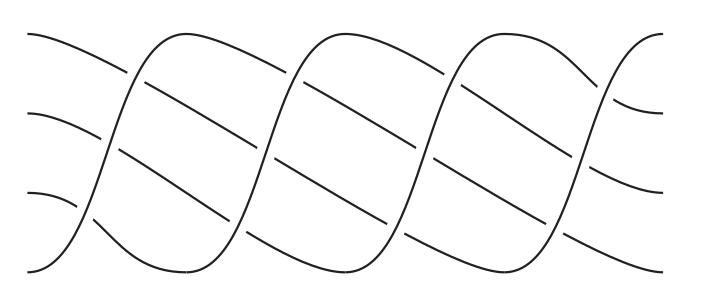
\includegraphics[width=6.5cm]{Images/volta_completa.png}
		\end{center}\caption{A volta completa, $\Delta_n^2$.}
		\label{full twist}
	\end{figure}
	
	\par\vspace{0.3cm} Da Figura \eqref{full twist}, podemos ver que $\Delta_n^2 = (\sigma_1\sigma_2\cdots\sigma_{n-1})^n$. Além disso, podemos também denotar por $\Delta_n$ a meia volta, e podemos escrevê-la em termos dos geradores $\sigma_i$ de $B_n$ da seguinte forma: $\Delta_n = (\sigma_1\sigma_2\cdots\sigma_{n-1})(\sigma_1\sigma_2\cdots\sigma_{n-2})\cdots(\sigma_2\sigma_1)\sigma_1$. Daí, como a notação sugere, $\Delta_n^2$ realmente é o quadrado de uma trança (e também a raiz $n$-ésima de uma trança, como podemos ver da Figura \eqref{full twist}).
	
	\par\vspace{0.3cm} Em particular, note que a meia volta não comuta, em geral, com os geradores de $B_n$, uma vez que $\Delta_n\sigma_2\neq\sigma_2\Delta_n$, por exemplo. De fato, o que ocorre é que $\sigma_i\Delta_n = \Delta_n\sigma_{n-i}$, ou seja, o cruzamento $\sigma_i$ ``desliza'' (é claro que se $n$ é par e $i=n/2$, então $\Delta_n$ comuta com $\sigma_i$).
	
	\begin{figure}[H]
		\label{delta5}
		\begin{center}	
			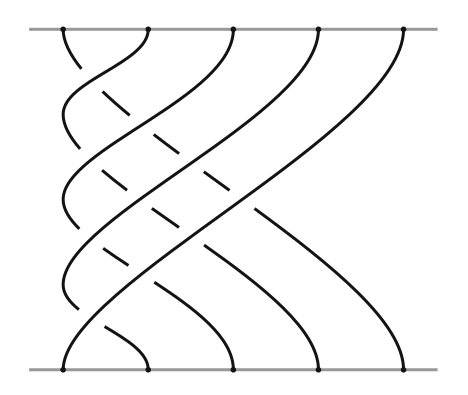
\includegraphics[width=6cm]{Images/delta5.png}
		\end{center}\caption{Diagrama de $\Delta_5$. Podemos ver que o cruzamento $\sigma_{i}$ ``desliza'', se tornando $\sigma_{n-i}$.}
	\end{figure}
	
	
	%\begin{center}
	%	\begin{tikzpicture}
	%	\label{delta}
	%	\braid[braid colour=black,strands=5,braid start={(0,0)}]	{\sigma_2\sigma_1 \sigma_2 \sigma_3\sigma_4\sigma_1\sigma_2\sigma_3\sigma_1\sigma_2\sigma_1}
	%	\node[font=\Huge] at (5.5,-5.5) {\(=\)};
	%	\braid[strands=5,braid start={(5,0)}]
	%	{\sigma_1 \sigma_2 \sigma_3\sigma_4\sigma_1\sigma_2\sigma_3\sigma_1\sigma_2\sigma_1\sigma_3}
	%	\end{tikzpicture}
	%\end{center}
	
	\par\vspace{0.3cm} Contudo, $\Delta_n^2$ comuta com toda trança de $B_n$, como é mostrado abaixo.
	
	\begin{proof}
		%Queremos mostrar que $\forall\beta\in B_n$, $\Delta_n^2\beta = \beta\Delta_n^2$. Isso equivale a mostrar que $\Delta_n^2\sigma_i = \sigma_i\Delta_n^2$. Por outro lado, como mostrado na Proposição \eqref{sigma1 e alfa geram B_n}, todo gerador de $B_n$ pode ser escrito em termos de $\sigma_1$ e $\alpha = \sigma_1\sigma_2\cdots\sigma_{n-1}$. Como $\alpha$ comuta com $\alpha^n = \Delta_n^2$, basta mostrarmos que $\sigma_1$ comuta com $\alpha^n$.
		
		
		
		Primeiro, note que $\sigma_i\Delta_n = \Delta_n\sigma_{n-i}$, como ilustram os diagramas acima. Daí, temos
		
		\begin{equation*}
		\sigma_i\Delta_n^2 = \sigma_i\Delta_n\Delta_n = \Delta_n\sigma_{n-i}\Delta_n = \Delta_n^2\sigma_i
		\end{equation*}
		
		\par\vspace{0.3cm} ou seja, $\Delta_n^2$ comuta com todo gerador de $B_n$ e, consequentemente, com toda trança de $B_n$.
		
		\par\vspace{0.3cm} 
		
	\end{proof}
	
	\par\vspace{0.3cm} Ora! Então $\Delta_n^2$ pertence ao centro de $B_n$. Na verdade, é possível mostrar que $\Delta_n^2$ gera o centro de $B_n$ para $n\geq 3$, i.e.
	
	
	\begin{theorem}
		\label{centro de B_n}
		Se $n\geq 3$, então $Z(B_n) = Z(P_n) = \langle \Delta_n^2 \rangle = \langle (\sigma_1\sigma_2\cdots\sigma_{n-1})^n \rangle$.
	\end{theorem}
	
	\par\vspace{0.3cm} Em outras palavras, toda trança do centro de $B_n$ é uma potência de $\Delta_n^2$.%, isto é, toda trança que comuta com todas as outras é uma potência da volta completa.
	
	\par\vspace{0.3cm} Demonstramos o Teorema \eqref{centro de B_n} para $n=3$.
	
	\begin{prop}
		$Z(B_3) = \langle (\sigma_1\sigma_2)^3 \rangle$
	\end{prop}
	
	\begin{proof}
		Primeiro, note que $(\sigma_1\sigma_2)^3\sigma_1 = \sigma_1\sigma_2\sigma_1\sigma_2\sigma_1\sigma_2\sigma_1 = \sigma_1(\sigma_1\sigma_2\sigma_1\sigma_2\sigma_1\sigma_2) = \sigma_1(\sigma_1\sigma_2)^3$ e também que $(\sigma_1\sigma_2)^3\sigma_2 = \sigma_1\sigma_2\sigma_1\sigma_2\sigma_1\sigma_2\sigma_2 = \sigma_2(\sigma_1\sigma_2\sigma_1\sigma_2\sigma_1\sigma_2) = \sigma_2(\sigma_1\sigma_2)^3$. Portanto, $\langle (\sigma_1\sigma_2)^3 \rangle\subseteq Z(B_3)$.
		
		\par\vspace{0.3cm} Agora, seja $g\in Z(B_3)$. Então, devemos ter, necessariamente, $g\sigma_1 = \sigma_1g$ e $g\sigma_2 = \sigma_2g$. Suponha, então, $g = \sigma_1^i\sigma_2^j$. Daí, temos
		
		\begin{align*}
		\begin{cases}
		\sigma_1^i\sigma_2^j\sigma_1 = \sigma_1^{i+1}\sigma_2^j \\
		\sigma_1^i\sigma_2^{j+1} = \sigma_2\sigma_1^{i}\sigma_2^j
		\end{cases} \Rightarrow \begin{cases}
		\sigma_2^j\sigma_1 = \sigma_1\sigma_2^j \\
		\sigma_1^i\sigma_2 = \sigma_2\sigma_1^i
		\end{cases} \Rightarrow i = j = 0 
		\end{align*} 
		
		\par\vspace{0.3cm} Suponha, agora, $g = (\sigma_1\sigma_2)^i$, $i\neq 0$. Então, temos
		
		\begin{align*}
		\begin{cases}
		(\sigma_1\sigma_2)^i\sigma_1 = \sigma_1(\sigma_1\sigma_2)^i \\
		(\sigma_1\sigma_2)^i\sigma_2 = \sigma_2(\sigma_1\sigma_2)^i
		\end{cases} \Rightarrow i = 3k, k\in\mathbb{Z}
		\end{align*}
		
		\par\vspace{0.3cm} A última implicação se deve ao seguinte raciocínio. A quantidade de termos no produto $(\sigma_1\sigma_2)^i\sigma_1$ é $2i+1$. Para transformar $(\sigma_1\sigma_2)^i\sigma_1$ em $\sigma_1(\sigma_1\sigma_2)^i$, devemos manipular os $2i$ termos de $\sigma_2(\sigma_1\sigma_2)^{i-1}\sigma_1$ usando a relação $\sigma_1\sigma_2\sigma_1 = \sigma_2\sigma_1\sigma_2$ para chegar em $(\sigma_1\sigma_2)^i$. Ora! Mas para utilizar a relação, precisamos de blocos de $3$ geradores, ou seja, devemos ter $i\in\mathbb{Z}$ tal que $\displaystyle{\frac{2i}{3}\in\mathbb{Z}}$. Como $2$ e $3$ são relativamente primos, devemos ter $i$ múltiplo de $3$.
		\par Por exemplo, $$\sigma_2(\sigma_1\sigma_2)^{4-1}\sigma_1 = \sigma_2\sigma_1\sigma_2\sigma_1\sigma_2\sigma_1\sigma_2\sigma_1 = \sigma_1\sigma_2\sigma_1\sigma_2\sigma_1\sigma_2\sigma_2\sigma_1 = (\sigma_1\sigma_2)^3\sigma_2\sigma_1\neq(\sigma_1\sigma_2)^4.$$
		
		\par\vspace{0.3cm} Daí, concluímos que todo elemento do centro de $B_3$ é uma potência de $(\sigma_1\sigma_2)^3$, ou seja, $Z(B_3)\subseteq\langle (\sigma_1\sigma_2)^3 \rangle$.
		
		\par\vspace{0.3cm} Portanto, $Z(B_3) = \langle (\sigma_1\sigma_2)^3 \rangle$.
		
	\end{proof}
	
	\begin{prop}
		Mostre que $l(\Delta_n^2) = n(n-1)$, sendo $l$ a função homomorfismo de comprimento definida no Lema \eqref{homomorfismo de comprimento} e $\Delta_n^2$ a volta completa em $B_n$.
	\end{prop}
	
	\begin{proof}
		Escrevendo $\Delta_n^2 = (\sigma_1\sigma_2\cdots\sigma_{n-1})^n$, segue da definição de $l$ que $l(\Delta_n^2) = n(n-1)$. 
		
		\par\vspace{0.3cm} Também podemos escrever $l(\Delta_n^2) = 2l(\Delta_n)$ e, como $\Delta_n = (\sigma_1\sigma_2\cdots\sigma_{n-1})(\sigma_1\sigma_2\cdots\sigma_{n-2})\cdots(\sigma_1\sigma_2)\sigma_1$, então $l(\Delta_n^2) = 2\Big( (n-1) + (n-2) + \cdots + 2 + 1 \Big) 2\Big( \displaystyle{\frac{n(n-1)}{2}} \Big) = n(n-1)$.
		
	\end{proof}
	
	%\begin{remark}
	%	No Teorema \eqref{centro de B_n}, usamos o fato de que $Z(B_n) = Z(P_n)$. Isso se deve ao fato de que $P_n$ é homomorfo a $B_n$, logo (como um homomorfismo preserva a operação) o centro de $B_n$ é levado no centro de $P_n$.
	%\end{remark}
	
	
	
	%\begin{theorem}
	%	$B_n$ e todos seus subgrupos são residualmente finitos.
	%\end{theorem}
	
	\par\vspace{0.3cm} Por fim, seja $f_n: P_n\to P_{n-1}$. Essa função é um homomorfismo sobrejetor, chamada \textit{homomorfismo esquecido}. A função $f_n$ pega uma trança em $P_n$, retira a $n$-ésima corda e a mapeia à trança resultante em $P_{n-1}$.
	\par\vspace{0.3cm} Para $n\geq 2$, definimos $U_n\vcentcolon=\Ker(f_n: P_n\to P_{n-1})$. Do diagrama do gerador de Artin, $A_{i,j}$, fica claro que $A_{i,n}\in U_n$, com $1\leq i\leq n-1$. 
	
	\begin{theorem}
		\label{U_n livre nos geradores de Artin}
		Para todo $n\geq 2$, $U_n$ é livre nos $n-1$ geradores $\{ A_{i,n} \}_{i=1,2,\dots,n-1}$.
	\end{theorem}
	
	\par\vspace{0.3cm} Aceitaremos o Teorema \eqref{U_n livre nos geradores de Artin} sem demonstração. Contudo, um corolário interessante é o seguinte.
	
	\begin{corollary}
		\label{B_n residualmente finito}
		$B_n$ e seus subgrupos são residualmente finitos.
	\end{corollary}
	
	\begin{proof}
		Um grupo $G$ é dito residualmente finito se para todo $\beta\in G-\{1\}$ existe um homomorfismo $f$ de $G$ em um grupo finito tal que $f(\beta)\neq 1$.
		\par\vspace{0.3cm} Sabemos que grupos livres são residualmente finitos e que o produto semidireto de dois grupos finitamente gerados e residualmente finitos é também residualmente finito.
		\par\vspace{0.3cm} Também sabemos, do Teorema \eqref{subgrupos normais e nucleos}, que $U_n\vartriangleleft P_n$. Da Definição \eqref{produto semidireto}, temos $P_n\cong U_n\rtimes P_{n-1}$. Tanto $U_n$ quanto $P_{n-1}$ são finitamente gerados e do Teorema \eqref{U_n livre nos geradores de Artin}, $U_n$ é residualmente finito. Daí, por indução em $n$, o Teorema \eqref{U_n livre nos geradores de Artin} implica $P_n$ residualmente finito.
		\par\vspace{0.3cm} Note que qualquer extensão de um grupo residualmente finito $P$ por um grupo finito é residualmente finita. Como $B_n$ é uma extensão de $P_n$ por $S_n$ e $P_n$ é residualmente finito, concluímos que $B_n$ também é.
		\par\vspace{0.3cm} Por fim, observe que todos os subgrupos de um grupo residualmente finito são também residualmente finitos.	
	\end{proof}
	\section{Tranças como espaços de configuração}\label{secao trancas como espacos de configuracao}
	\hspace{12pt} Há varias conexões entre grupos de tranças e topologia, e uma delas envolve \textit{espaços de configuração}, que nada mais são do que um espaço que contém todos os estados possíveis de um sistema. Por vezes, espaços de configuração são chamados de \textit{espaços de estado} ou \textit{espaços de parâmetros}.
	\par\vspace{0.3cm} Por exemplo, podemos usar um espaço de configuração para modelar o movimento coletivo de vários objetos, como carros nas ruas de uma cidade ou pacotes em uma \textit{network} ou moléculas em uma solução ou ainda robôs em uma fábrica.
	\par\vspace{0.3cm} Para um exemplo mais concreto, considere o seu braço. Nele, há três juntas: uma no ombro, uma no cotovelo e uma no pulso. Tanto o seu ombro quanto o seu pulso têm dois graus de liberdade (i.e., podem girar em dois sentidos diferentes), enquanto que o seu cotovelo tem apensa um grau de liberdade, totalizando cinco dimensões de configuração.
	\par\vspace{0.3cm} Um braço robótico modelado a partir do seu braço tem de navegar por um espaço de configuração cinco-dimensional para poder aproveitar toda a flexibilidade existente nesse sistema de juntas. Para ilustrar, imagine que ao invés de uma mão, você tem uma plataforma rígida conectada ao seu pulso e suponha que você queira levantar um copo d'água de abaixo da sua cintura até acima do seu ombro. Isso não será possível de fazer com a plataforma rígida no lugar da mão, porque apenas a rotação do ombro não é suficiente para fazer o movimento desejado (isso é o que os bebês fazem, e eles derramam a água sempre).
	\par\vspace{0.3cm} Mas qual a conexão entre espaços de configuração e grupos de trança? Bom, até agora, falamos de tranças individuais como objetos topológicos, como indicam as Definições \eqref{def geometrica tranca} e \eqref{outra def geometrica tranca}. Contudo, os grupos de trança em si também são objetos topológicos, no sentido de que cada grupo de trança descreve, de forma natural, os diferentes tipos de \textit{loops} que existem em um certo espaço de configuração. O espaço em questão modela o movimento coletivo de $n$ partículas distintas no plano que não podem colidir.
	\par\vspace{0.3cm} Então, imagine $n$ partículas no plano e estenda esse plano para formar a parede esquerda de uma trança. Agora, deslize o plano da esquerda para a direita, e imagine que cada partícula deixa um rastro à medida que o plano se move. O que acontece?
	\par\vspace{0.3cm} Bom, se as partículas ficam paradas (no plano), então quando o plano parar, você terá $n$ trilhas paralelas: a trança identidade! 
	
	
	\begin{figure}[H]
		\begin{center} 
			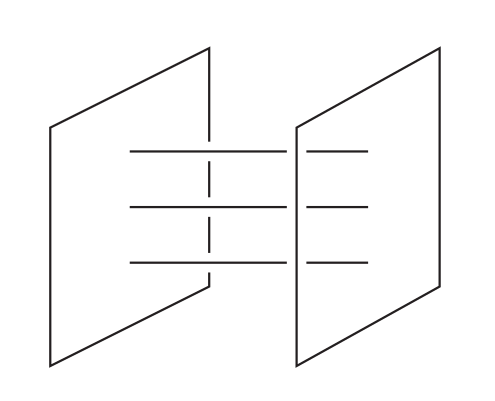
\includegraphics[width=9cm]{Images/tranca_identidade_conf.png}
		\end{center}\caption{A trança identidade em um espaço de configuração}\label{tranca identidade espaco configuracao}
	\end{figure}
	
	\par\vspace{0.3cm} Entretanto, se as partículas se movem no plano à medida que eles desliza, o que ocorre? Bom, desde que nenhum par de partículas colida, veremos uma trança! E claramente toda trança pode ser feita desse modo. Veja a figura abaixo. Note que estamos visualizando a direção $x$ como o eixo temporal.
	\par\vspace{0.3cm} Para um exemplo mais visual, podemos observar o movimento dos planetas do Sistema Solar, como nesse vídeo.\footnote{ \url{https://www.youtube.com/watch?v=0jHsq36_NTU&list=WL&index=2&t=50s}} 
	
	\begin{figure}[H]
		\begin{center}
			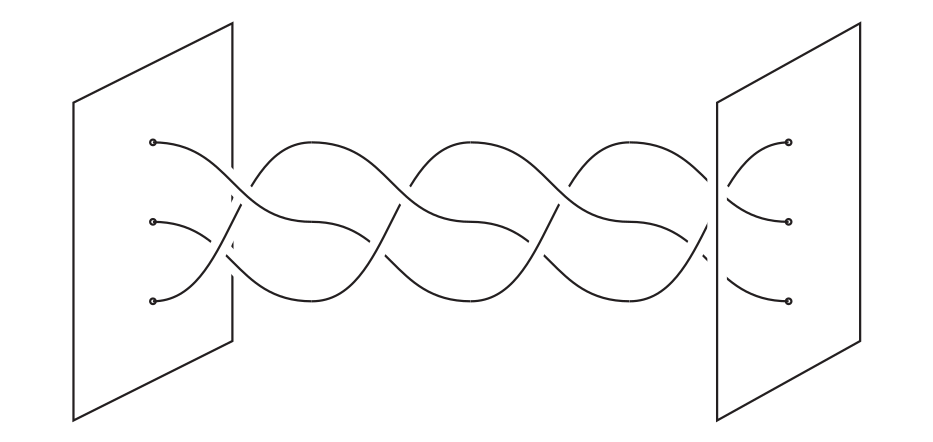
\includegraphics[width=10cm]{Images/tranca_conf.png}
		\end{center}\caption{Uma trança não trivial em um espaço de configuração.}\label{tranca espaco configuracao}
	\end{figure} 
	%\newpage
	\par\vspace{0.3cm} Para fazermos o produto de duas tranças usando essa ideia, precisamos ter certeza de que o coletivo de partículas no final da trança está no mesmo lugar que no começo da trança, pois assim podemos concatenar duas tranças sem haver nenhuma descontinuidade no meio.
	\par\vspace{0.3cm} A posição inicial é uma \textit{configuração} de $n$ partículas. O conjunto de todas as configurações possíveis é o espaço de configuração
	\begin{align}
	C_n(\mathbb{R}^2) = \{ (p_1, \dots, p_n)\in (\mathbb{R}^2)^n | p_i\neq p_j \text{ para }i\neq j \} 
	\label{configuracao ordenada}
	\end{align}
	\par\vspace{0.3cm} em que a condição $p_i\neq p_j$ indica a necessidade de um par partículas não colidirem.
	\par\vspace{0.3cm} O que definimos em \eqref{configuracao ordenada} foi o conjunto de configurações \textit{ordenadas}. Como o nosso propósito é descrever tranças, gostaríamos de ignorar a ordem e apenas focar no conjunto de partículas, e.g., queremos considerar $(p_1, p_2)$ como o mesmo que $(p_2, p_1)$ e pensar em ambos apenas como $\{p_1, p_2\}$. Para isso, definimos a versão não ordenada:
	\begin{align}
	UC_n(\mathbb{R}^2) = \{ \{ p_1, \dots, p_n\}\subset\mathbb{R}^2| p_i\neq p_j \text{ para }i\neq j  \}\label{configuracao nao ordenada}
	\end{align} 
	\par\vspace{0.3cm} ou, em palavras, o conjunto de subconjuntos de $n$ pontos do plano. 
	\par\vspace{0.3cm} Podemos também denotar $C_n(\mathbb{R}^2)$ por $\mathbb{F}_n(\mathbb{R}^2)$ e $UC_n(\mathbb{R}^2)$ por $\widetilde{\mathbb{F}}_n(\mathbb{R}^2)$, sendo $\sim$ a relação de equivalência cujas classes são os conjuntos de permutações de um dado ponto em $(\mathbb{R}^2)^n$. 
	\par\vspace{0.3cm} De forma geral, se $\mathbb{M}$ é uma variedade de dimensão maior ou igual a 2, então $\mathbb{F}_n(\mathbb{M})$ denota o subespaço de $\mathbb{M}^{(n)}$ definido por
	\begin{align}
	\mathbb{F}_n(\mathbb{M}) = \{ (x_1, \dots, x_n)\in \mathbb{M}^{(n)} | x_i\neq x_j \text{ para }i\neq j \} 
	\label{espaco de configuracao de M}
	\end{align}
	\par\vspace{0.3cm} Esse subespaço é chamado \textit{espaço de configuração} de $\mathbb{M}$. Sendo $\sim$ a mesma relação de equivalência definida acima, o espaço quociente $^{\displaystyle{\mathbb{F}_n(\mathbb{M})}}/_{\sim}$, que também pode ser denotado por $\widetilde{\mathbb{F}}_n(\mathbb{M})$, é definido por
	\begin{align}
	\widetilde{\mathbb{F}}_n(\mathbb{M}) = \{ \{ x_1, \dots, x_n\}\subset\mathbb{M}| x_i\neq x_j \text{ para }i\neq j  \}\label{espaco de configuracao nao ordenado de M}
	\end{align} 
	\par\vspace{0.3cm} Pelo modo como definimos $\sim$ acima, podemos ver que $UC_n(\mathbb{R}^2) = \displaystyle{C_n(\mathbb{R}^2)}/\displaystyle{S_n}$. Agora, voltando na Figura \eqref{tranca espaco configuracao}, tanto a parede da esquerda quando a parede da direita representam pontos de $UC_3(\mathbb{R}^2)$. Na verdade, as duas paredes representam o mesmo ponto (mas não o mesmo ponto de $C_3(\mathbb{R}^2)$, pois a configuração final é $(p_2, p_3, p_1)$, sendo $p_1$ o ponto inferior e $p_3$ o ponto superior). 
	\par\vspace{0.3cm} Além disso, quando deslizamos a parede da esquerda para a direita de forma a criar a trança, em cada instante de tempo temos um ponto de $UC_3(\mathbb{R}^2)$. Isso se deve ao fato de que cada corda é monotônica. Em outras palavras, podemos ver a trança como um \textit{loop} em $UC_3(\mathbb{R}^2)$.
	\par\vspace{0.3cm} Para fixar, podemos pensar em esquerda-direita como o eixo temporal, e então a trança tridimensional toda é como um filme de três partículas dançando no plano bidimensional (sem colidir) e retornando ao lugar onde começaram.
	\par\vspace{0.3cm} Equivalentemente, a trança é o gráfico de uma função $[0,1]\to UC_3(\mathbb{R}^2)$, cujos pontos inicial e final concordam. Ou seja, podemos pensar em tranças como \textit{loops} de configurações. De fato, essa é, essencialmente, uma correspondência injetiva.
	\par\vspace{0.3cm} Antes de prosseguir, definimos (informalmente) o conceito de grupo fundamental.
	
	\begin{deff}
		\label{def informal grupo fundamental}
		Dado um espaço topológico $X$ e um ponto $x_0\in X$, o conjunto de loops que começam e terminam em $x_0$ e que são caminhos fechados em $X$ é chamado grupo fundamental de $X$ com ponto base $x_0$ e denotado por $\pi_1(X,x_0)$.
	\end{deff}
	
	\par\vspace{0.3cm} Um detalhe importante é que se $X$ é conexo por caminhos (i.e., dado um par de pontos em $X$, existe um caminho totalmente contido em $X$ que liga esses dois pontos), então a escolha do ponto base não faz diferença. Esse é o nosso caso, e então denotaremos o grupo fundamental de $X$ por $\pi_1(X)$ apenas.
	\par\vspace{0.3cm} Com a Definição \eqref{def informal grupo fundamental}, podemos enunciar o seguinte teorema.
	
	\begin{theorem}
		\label{grupo fundamental de tranca}
		O grupo fundamental $\pi_1(UC_n(\mathbb{R}^2))$ é isomorfo ao grupo de trança $B_n$, e o grupo fundamental $\pi_1(C_n(\mathbb{R}^2))$ é isomorfo ao grupo de tranças puras $P_n$.
	\end{theorem} 
	
	\par\vspace{0.3cm} Da Definição \eqref{def informal grupo fundamental}, podemos ver que o grupo fundamental trata sobre os diferentes \textit{loops} em um espaço topológico. A noção de equivalência de \textit{loops} (i.e., homotopia, que nada mais é que uma deformação contínua de um caminho para outro) se traduz diretamente para nossa noção de equivalência de tranças.
	\par\vspace{0.3cm} Portanto, o Teorema \eqref{grupo fundamental de tranca} nos diz não só que tranças podem ser vistas como \textit{loops} em um espaço de configuração, mas também que podemos construir todos os \textit{loops} nesse espaço de configuração dessa maneira.
	\par\vspace{0.3cm} Além de nos proporcionar um outro modo de pensar em tranças, essa perspectiva topológica é útil tanto para provar coisas sobre tranças quanto para realizar generalizações interessantes. Por exemplo, é possível demonstrar o Teorema \eqref{apresentacao de B_n} usando essas ideias. 
	\par\vspace{0.3cm} Para outro exemplo, observe que a própria notação, $C_n(\mathbb{R}^2)$ sugere uma generalização óbvia, de substituir $\mathbb{R}^2$ por outros espaços topológicos, como superfícies, grafos ou variedades. Da mesma forma, o conjunto de (classes de equivalência de) \textit{loops} em um espaço de configuração de $n$ partículas em um espaço topológico $X$ é chamado de \textit{grupo de trança associado a $X$}.
	\par\vspace{0.3cm} Em símbolos, escrevemos $\pi_1(UC_n(X)) = B_n(X)$ e $\pi_1(C_n(X)) = P_n(X)$. Desse modo, os grupos usuais $B_n$ e $P_n$ são, na verdade, $B_n(\mathbb{R}^2)$ e $P_n(\mathbb{R}^2)$.
	\par\vspace{0.3cm} Por exemplo, sendo $X = \mathbb{R}$ e tomando $n=2$, temos que
	\begin{align*}
	UC_2(\mathbb{R}) = \big\{  \{p_1,p_2\}\subset\mathbb{R}|p_1\neq p_2  \big\} \\
	C_2(\mathbb{R}) = \big\{ (p_1,p_2)\in\mathbb{R}^2|p_1\neq p_2 \big\}
	\end{align*}
	\par\vspace{0.3cm} ou seja, os espaços de configuração não ordenado e ordenado, respectivamente, de dois pontos em uma reta. Não é difícil perceber que tanto $C_2(\mathbb{R})$ quanto $UC_2(\mathbb{R})$ possuem 3 componentes conexos e, em geral, $C_n(\mathbb{R})$ e $UC_n(\mathbb{R})$ possuem $n+1$ componentes conexos. Também podemos tomar $X = \mathbb{S}^1$, ou seja, uma circunferência. Nesse caso, $C_n(\mathbb{S}^1)$ e $UC_n(\mathbb{S}^1)$ têm $n$ componentes conexos.
	\par\vspace{0.3cm} Agora, vamos considerar $X = \mathbb{S}^2$, a esfera em $\mathbb{R}^3$. Nesse caso, $B_n(X) = B_n(\mathbb{S}^2)$ é chamado de \textit{grupo de tranças esféricas}. Uma primeira pergunta natural seria: qual a diferença entre tranças esféricas e ``tranças planares''? Bom, podemos imaginar as paredes dos diagramas das tranças planares como sendo pequenos pedaços de esferas enormes, por exemplo, como mostra a figura \eqref{diagrama tranca esferica}abaixo (na verdade, essa ideia pode ser aplicada a tranças em qualquer superfície, não apenas na esfera).
	
	\begin{figure}[H]
		\begin{center}
			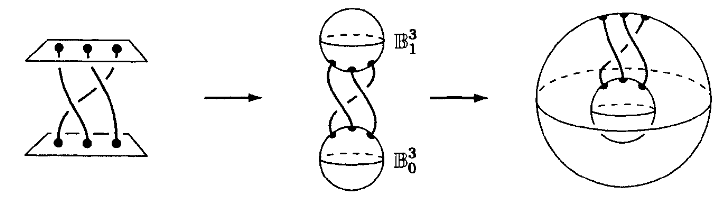
\includegraphics[width=12cm]{Images/diagrama_tranca_esferica.png}
		\end{center}\caption{Diagrama de uma trança esférica}
		\label{diagrama tranca esferica}
	\end{figure}
	\par\vspace{0.3cm} Logo, temos de modo natural a função $f: B_n(\mathbb{R}^2)\to B_n(\mathbb{S}^2)$. Não é muito difícil perceber que podemos obter toda trança esférica a partir de uma trança planar, i.e., que $f$ é sobrejetora. Contudo, $f$ não é injetora.
	\par\vspace{0.3cm} Isso se deve ao fato de que, para tranças esféricas, as cordas podem ser deformadas de modo a ``darem a volta'', como mostra a figura a seguir. Podemos pensar em $B_n(\mathbb{R}^2)$ como tranças dentro de um cubo, ficando ``presas'' lá dentro e, portanto, impossibilitadas de realizar movimentos como os que estão abaixo.
	
	\begin{figure}[H]
		\begin{center}
			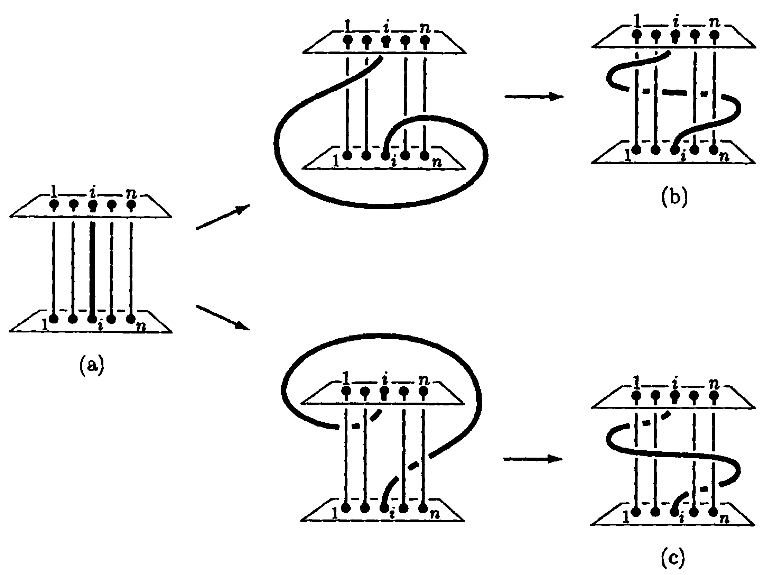
\includegraphics[width=10cm]{Images/movimentos_trancas_esfericas.png}
		\end{center}\caption{Movimentos possíveis para tranças esféricas, mas impossíveis para tranças planares}
		\label{movimentos trancas esfericas}
	\end{figure} 
	
	\par\vspace{0.3cm} Como os geradores $\sigma_i$ de $B_n(\mathbb{R}^2)$ também são geradores de $B_n(\mathbb{S}^2)$, as relações das tranças planares continuam válidas para as tranças esféricas. Contudo, os novos movimentos mostrados na Figura \eqref{movimentos trancas esfericas} nos dão uma nova relação em $B_n(\mathbb{S}^2)$, a saber
	\begin{align}
	\sigma_{i-1}\sigma_{i-2}\cdots\sigma_2\sigma_1^2\sigma_2\sigma_3\cdots\sigma_{n-2}\sigma_{n-1}^2\sigma_{n-2}\sigma_{n-3}\cdots\sigma_i = 1
	\label{novas relacoes}
	\end{align}
	\par\vspace{0.3cm} Contudo, toda relação, para $i=1,2\dots,n-1$, em \eqref{novas relacoes} é consequência da única relação
	\begin{align}
	(\sigma_1\sigma_2\cdots\sigma_{n-1})(\sigma_{n-1}\sigma_{n-2}\cdots\sigma_1) = 1
	\label{nova relacao}
	\end{align}
	\par\vspace{0.3cm} De fato, essa relação é dada pelo mesmo movimento que o diagrama (b) da Figura \eqref{movimentos trancas esfericas}, mas com a corda $1$ indo para a direita, como o diagrama abaixo.
	\begin{center}
		\begin{tikzpicture}
		\braid[braid colour=black,strands=4,braid start={(0,0)}]	{\sigma_1\sigma_2\sigma_3\sigma_3\sigma_2\sigma_1}
		%\node[font=\Huge] at (4.5,-1.0) {\(\neq\)};
		%\braid[strands=3,braid start={(5,0)}]
		%{\sigma_2\sigma_1}
		
		%gama em $B_4(\mathbb{S}^2)$
		\end{tikzpicture}
	\end{center}
	\par\vspace{0.3cm} Portanto, uma apresentação de $B_n(\mathbb{S}^2)$ tem os mesmos geradores e relações que $B_n(\mathbb{R}^2)$, mas com a última relação em \eqref{nova relacao}. De fato, essa é a apresentação completa de $B_n(\mathbb{S}^2)$, conforme o teorema abaixo, que não será demonstrado.
	
	\begin{theorem}
		\label{apresentacao de B_n(S^2)}
		O grupo de tranças esféricas $B_n(\mathbb{S}^2)$ tem apresentação	
		\begin{align*}
		B_n(\mathbb{S}^2) = \langle \sigma_1, \sigma_2, \dots, \sigma_{n-1}|&\sigma_i\sigma_j = \sigma_j\sigma_i, \text{ para } |i - j|>1, \\ 
		&\sigma_i\sigma_{i+1}\sigma_i = \sigma_{i+1}\sigma_i\sigma_{i+1}, \text{ para } 1\leq i\leq n-2 , \\
		&\sigma_1\sigma_2\cdots\sigma_{n-2}\sigma_{n-1}^2\sigma_{n-2}\cdots\sigma_2\sigma_1 = 1  \rangle.
		\end{align*} 
	\end{theorem}  
	
	\par\vspace{0.3cm} Então, voltando à nossa função $f$: ela não é injetora, pois a trança em \eqref{nova relacao} pertence ao núcleo de $f$, ou seja, $\Ker f$ não é trivial. Outra trança que pertence ao núcleo de $f$ é $\displaystyle{(\Delta_n^2)^2}$, o quadrado da volta completa, que tem ordem $2$ em $B_n(\mathbb{S}^2)$.
	\par\vspace{0.3cm} Na verdade, esse fato pode ser generalizado no seguinte lema.
	
	\begin{lemma}
		\label{potencia da volta completa trivial}
		Para todo $n> 2$, a trança de Dirac $\delta = (\sigma_1\sigma_2\cdots\sigma_{n-1})^{kn} = (\Delta_n^2)^k$ é trivial em $B_n(\mathbb{S}^2)$ se, e só se, $k$ é par. 
	\end{lemma}
	
	\begin{proof}
		Já sabemos que $(\Delta_n^2)^2 = 1$ em $B_n(\mathbb{S}^2)$. Então, se $k$ é par, podemos escrever $k=2j$ e segue que $(\Delta_n^2)^k = [(\Delta_n^2)^2]^j = 1^j = 1$. Por outro lado, como $|\Delta_n^2| = 2$ em $B_n(\mathbb{S}^2)$, então $(\Delta_n^2)^k = 1$ implica que $2|k$, i.e, $k$ par.
	\end{proof}
	\par\vspace{0.3cm} Do Teorema \eqref{apresentacao de B_n(S^2)}, podemos obter alguns fatos interessantes sobre o grupo de tranças esféricas. Por exemplo, $B_2(\mathbb{S}^2) = \langle \sigma_1|\sigma_1^2=1 \rangle$, ou seja, $B_2(\mathbb{S}^2)$ é um grupo finito de ordem $2$ com um gerador: $\mathbb{Z}_2$. Além disso, também podemos definir o homomorfismo de comprimento que definimos para as tranças planares, mas com uma pequena alteração.
	
	\begin{prop}
		\label{homomorfismo de comprimento em trancas esfericas}
		Seja $\beta\in B_n(\mathbb{S}^2)$. Tomando $\beta = \sigma_{i_1}^{\varepsilon_1}\cdots\sigma_{i_k}^{\varepsilon_k}$, sendo $\varepsilon_i = \pm1$ para $i=1,2,\dots,k$, então podemos definir a função $l$, chamada \textit{homomorfismo de comprimento}, de $B_n(\mathbb{S}^2)$ em $\mathbb{Z}$ como	
		\begin{align*}
		l(\beta) = \sum_{i=1}^{k}\varepsilon_i\text{ }\mathrm{mod}(2(n-1))
		\end{align*}
		\par\vspace{0.3cm} ou seja, a soma dos expoentes módulo $2(n-1)$. Então, $l$ é invariante em $B_n(\mathbb{S}^2)$, i.e., se $\beta = \beta'$ em $B_n(\mathbb{S}^2)$, então $l(\beta) = l(\beta')\text{ }\mathrm{mod}(2(n-1))$.
	\end{prop}
	
	\begin{proof}
		Do Teorema \eqref{apresentacao de B_n(S^2)}, sabemos todas as relações de $B_n(\mathbb{S}^2)$. Para as duas primeiras, $l(\beta)$ é constante para cada uma dessas relações. Contudo, para a terceira relação, $l(\beta)$ difere por um fator de $\pm2(n-1)$ para os dois lados da relação. Como $l(1) = 0$ e $l$ está bem definida (demonstração análoga à do Lema \eqref{homomorfismo de comprimento}), devemos ter a igualdade módulo $2(n-1)$.
	\end{proof}
	
	\par\vspace{0.3cm} Por exemplo, como $l((\sigma_1\sigma_2)^3) = 6\neq 0\text{ }\mathrm{mod}4$ e $l(1) = 0$, então, em $B_3(\mathbb{S}^2)$, $(\sigma_1\sigma_2)^3\neq 1$. Outro exemplo: $\sigma_1^4=1$ em $B_3(\mathbb{S}^2)$, mas $\sigma_1^4\neq1$ em $B_4(\mathbb{S}^2)$. Esse exemplo nos mostra uma diferença notável entre $B_n(\mathbb{R}^2)$ e $B_n(\mathbb{S}^2)$, pois se $\beta$ é trivial em $B_m(\mathbb{R}^2)$ e $m\leq n$, então $\beta$ também é trivial em $B_n(\mathbb{R}^2)$, enquanto que para $B_m(\mathbb{S}^2)$ e $B_n(\mathbb{S}^2)$ isso, em geral, não é verdade.
	\par\vspace{0.3cm} Note também que a recíproca da Proposição \eqref{homomorfismo de comprimento em trancas esfericas} é falsa. Por exemplo, $\sigma_1^6\neq1$ em $B_4(\mathbb{S}^2)$ mas $l((\sigma_1)^6) = 0\text{ }\mathrm{mod}6 = l(1)$.
	\par\vspace{0.3cm} A apresentação no Teorema \eqref{apresentacao de B_n(S^2)} tem também uma interessante consequência, enunciada no Lema \eqref{B_3(S^2) tem ordem 12}. Antes, contudo, introduziremos um pequeno conceito, as \textit{transformações de Tietze}.
	\subsubsection{Transformações de Tietze}
	\hspace{12pt} Dada uma apresentação de um grupo $G$, temos os seguintes movimentos:
	\begin{enumerate}
		\item se uma relação pode ser deduzida a partir das relações existentes, então podemos adicionar essa nova relação à apresentação. Por exemplo, se $G = \langle x|x^3=1 \rangle$, obtemos a relação $x^6 = 1$ a partir de $x^3=1$. Logo, podemos escrever $G = \langle x|x^3=1,x^6=1 \rangle$.
		\item Reciprocamente, se uma relação da apresentação pode ser deduzida a partir das outras, então podemos removê-la. Em $G = \langle x|x^3=1,x^6=1 \rangle$, a relação $x^6=1$ pode ser deduzida de $x^3=1$ e, portanto, pode ser removida da apresentação. Contudo, note que não podemos remover $x^3=1$, pois teríamos outro grupo.
		\item Podemos adicionar um gerador escrito como uma palavra nos geradores originais. Começando com $G = \langle x|x^3=1 \rangle$ e fazendo $y=x^2$, a nova apresentação $G = \langle x,y|x^3=1,y=x^2 \rangle$ define o mesmo grupo.
		\item De modo semelhante, se podemos formar uma relação em que um dos geradores é uma palavra nos outros geradores, então esse gerador pode ser removido. Por exemplo, a apresentação do grupo abeliano de ordem $4$, $G = \langle x,y,z|x=yz, y^2=1, z^2=1, x=x^{-1} \rangle$ pode ser substituído por $G = \langle y,z|y^2=1,z^2=1,(yz)=(yz)^{-1} \rangle$.
	\end{enumerate}
	
	\par\vspace{0.3cm} Usaremos essas transformações para demonstrar o seguinte lema.
	
	\begin{lemma}
		\label{B_3(S^2) tem ordem 12}
		$B_3(\mathbb{S}^2)$ tem apresentação $\langle a,b|b^6=1,a^2=b^3=(ab)^2 \rangle$, sendo, portanto, isomorfo a $Q_6$, o grupo dicíclico de ordem $12$. 
	\end{lemma} 
	
	\begin{proof}
		Sabemos, do Teorema \eqref{apresentacao de B_n(S^2)}, que $B_3(\mathbb{S}^2) = \langle \sigma_1,\sigma_2 | \sigma_1\sigma_2\sigma_1 = \sigma_2\sigma_1\sigma_2\text{, } \sigma_1\sigma_2^2\sigma_1 = 1\rangle$. Fazendo $a = \sigma_1\sigma_2\sigma_1$ e $b = \sigma_1\sigma_2$, temos:
		
		\begin{align*}
		a^2 = \sigma_1\sigma_2\sigma_1\sigma_1\sigma_2\sigma_1 = \sigma_1\sigma_2\sigma_1\sigma_2\sigma_1\sigma_2 = (\sigma_1\sigma_2)^3 = b^3 \\
		(ab)^2 = \sigma_1\sigma_2\sigma_1\sigma_1\sigma_2\sigma_1\sigma_2\sigma_1\sigma_1\sigma_2 =  \sigma_1\sigma_2\sigma_1\sigma_2\underbrace{\sigma_1\sigma_2\sigma_2\sigma_1}_{1}\sigma_1\sigma_2 = (\sigma_1\sigma_2)^3 = b^3 \\
		b^6 = \sigma_1\sigma_2\sigma_1\sigma_2\sigma_1\sigma_2\sigma_1\sigma_2\sigma_1\sigma_2 = \underbrace{\sigma_1\sigma_2\sigma_2\sigma_1}_{1}\sigma_2\sigma_2\underbrace{\sigma_1\sigma_2\sigma_2\sigma_1}_{1}\sigma_2\sigma_2 = \sigma_2^4 
		\end{align*}
		
		\par\vspace{0.3cm} Vamos mostrar que tanto $\sigma_1$ quanto $\sigma_2$ têm ordem 4. Então, seja $N$ o fecho normal de $a^2$, i.e., $N = \{1,a\}$. Daí, $N\vartriangleleft B_3(\mathbb{S}^2)$ e, portanto, o grupo quociente $B_3(\mathbb{S}^2)/N$ tem apresentação $\langle a,b|a^2=b^3=(ab)^2=1 \rangle$, que é a apresentação de $S_3$, o grupo simétrico em $3$ elementos. Logo, $|B_3(\mathbb{S}^2)| = |N||S_3| = 12$.
		\par\vspace{0.3cm} Por fim, note que $(ab)^2 = a^2$ implica $a = b^{-1}ab^{-1}$, logo
		\begin{align*}
		\sigma_1^4 = (b^{-1}a)^4 = (b^{-1}ab^{-1})a(b^{-1}ab^{-1})a = a^4 = 1\text{ (observe o diagrama abaixo)}
		\end{align*}  
		
		\begin{figure}[H]
			\begin{center}
				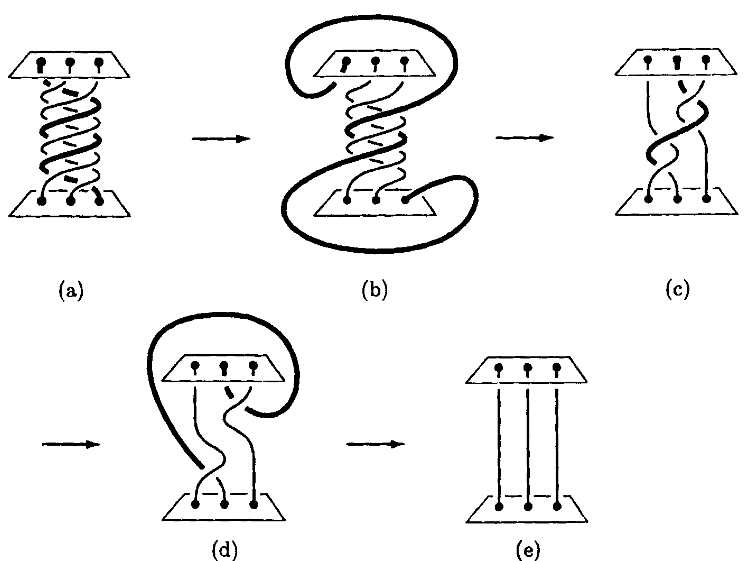
\includegraphics[width=12cm]{Images/manipulacao_de_a4.png}
			\end{center}\caption{$a^4 = 1$ em $B_3(\mathbb{S}^2)$}
		\end{figure}
		
		\par\vspace{0.3cm} Como $\sigma_1\neq 1$ e $\sigma_1^2\neq 1$, então, pela Proposição \eqref{homomorfismo de comprimento em trancas esfericas}, $|\sigma_1| = 4$.
		\par\vspace{0.3cm} Similarmente, $(ab)^2 = a^2$ implica $bab=a$ e também $ba=a^{-1}b^2$, logo
		\begin{align*}
		\sigma_2^4 = (a^{-1}b^2)^4 = (ba)^4 = (bab)a(bab)a = a^4 = 1
		\end{align*}
		\par\vspace{0.3cm} Como $\sigma_2\neq1$ e $\sigma_2^2\neq1$ então, da Proposição \eqref{homomorfismo de comprimento em trancas esfericas}, temos $|\sigma_2|=4$. 
		\par\vspace{0.3cm} Além disso, como $a^4 = 1$, temos $b^6=1$.
		\par\vspace{0.3cm} Por fim, da tabela \eqref{tabela grupos}, vemos que $B_3(\mathbb{S}^2)\cong Q_6$, o grupo dicíclico de ordem 12.
	\end{proof}
	
	\par\vspace{0.3cm} Do Lema \eqref{B_3(S^2) tem ordem 12}, podemos listar os elementos de $B_3(\mathbb{S}^2)$:
	\begin{align*}
	B_3(\mathbb{S}^2) = \left\{ 1, a, a^2, a^3, b, b^2, b^4, b^5, ab, ab^2, ab^4, ab^5 \right\}
	\end{align*}
	\par\vspace{0.3cm} Podemos ainda escrever esse elementos em termos dos geradores $\sigma_1$ e $\sigma_2$. Com algumas simplificações, obtemos:
	\begin{align*}
	B_3(\mathbb{S}^2) = \left\{ 1, \sigma_1\sigma_2\sigma_1, (\sigma_1\sigma_2\sigma_1)^2, (\sigma_1\sigma_2\sigma_1)^3, \sigma_1\sigma_2, (\sigma_1\sigma_2)^2, \sigma_1^3\sigma_2, \sigma_2\sigma_1, \sigma_1, \sigma_2^3, \sigma_2\sigma_1^3\sigma_2, \sigma_1^3 \right\}
	\end{align*}
	\par\vspace{0.3cm} Fazendo os diagramas, vemos que apenas $1$ e $(\sigma_1\sigma_2\sigma_1)^2 = a^2 = b^3$ são tranças puras. Além disso, como $a^4 = 1 = b^6$, concluímos que $P_3(\mathbb{S}^2) = \langle a^2 \rangle = \langle b^3 \rangle$.
	
	\par\vspace{0.3cm} Agora, vamos considerar $B_4(\mathbb{S}^2)$, que tem apresentação
	\begin{align*}
	B_4(\mathbb{S}^2) = \langle \sigma_1, \sigma_2, \sigma_3| &\sigma_1\sigma_2\sigma_1 = \sigma_2\sigma_1\sigma_2 \\ &\sigma_2\sigma_3\sigma_2 = \sigma_3\sigma_2\sigma_3 \\
	&\sigma_1\sigma_3 = \sigma_3\sigma_1\\
	&\sigma_1\sigma_2\sigma_3^2\sigma_2\sigma_1 = 1\rangle
	\end{align*}
	
	\par\vspace{0.3cm} Seja $N$ o fecho normal de $\sigma_1\sigma_3^{-1}$. Então, a apresentação do grupo quociente $G = B_4(\mathbb{S}^2)/N$, é obtida de $B_4(\mathbb{S}^2)$ adicionando a relação $\sigma_1\sigma_3^{-1} = 1$ ou, equivalentemente, $\sigma_1=\sigma_3$. O efeito dessa relação extra é reduzir o número de relações para duas, a saber
	\begin{center}
		\begin{tabular}{ccc}
			$\sigma_1\sigma_2\sigma_1 = \sigma_2\sigma_1\sigma_2$ & e & $\sigma_1\sigma_2\sigma_1^2\sigma_2\sigma_1 = 1$ \\
		\end{tabular}
	\end{center}
	
	\par\vspace{0.3cm} A última relação pode ser manipulada como a seguir:
	\begin{align*}
	1 &= \sigma_1\sigma_2\sigma_1\sigma_1\sigma_2\sigma_1 \\
	&= \sigma_1\sigma_2\sigma_1\sigma_2\sigma_1\sigma_2 \\ 
	&= (\sigma_1\sigma_2)^3  
	\end{align*}
	\par\vspace{0.3cm} Portanto, $G = \langle \sigma_1, \sigma_2| \sigma_1\sigma_2\sigma_1=\sigma_2\sigma_1\sigma_2\text{, } (\sigma_1\sigma_2)^3=1 \rangle$. Como antes, tome $a = \sigma_1\sigma_2\sigma_1$ e $b = \sigma_1\sigma_2$. Como $\sigma_1 = b^{-1}a$ e $\sigma_2 = a^{-1}b^2$, as relações de $G$ se tornam $a^2 = b^3$ e $b^3 = 1$, logo $G = \langle a,b|a^2=b^3=1 \rangle$. Vamos mostrar que $G$ é infinito, usando o seguinte lema, que será aceito sem demonstração.
	
	\begin{lemma}
		\label{grupo triangular}
		O grupo triangular, ou grupo de Dyck, $T(l,m,n) = \langle a,b|a^l=b^m=(ab)^n=1 \rangle$ é finito se, e só se, $\displaystyle{\frac{1}{l} + \frac{1}{m} + \frac{1}{n} - 1 > 0}$.
	\end{lemma}
	
	
	\begin{prop}
		\label{quociente de B4(S2) infinito}
		$G = \langle a,b|a^2=b^3=1 \rangle$ é infinito e, consequentemente, $B_4(\mathbb{S}^2)$ é infinito.
	\end{prop}
	
	\begin{proof}
		Seja $\widehat{G} = \langle a,b|a^2=b^3=(ab)^7=1 \rangle$. Note que $\widehat{G}$ é um grupo quociente de $G$ e, além disso, $\widehat{G} = T(2,3,7)$. Do Lema \eqref{grupo triangular}, temos $\widehat{G}$ infinito, pois $\displaystyle{\frac{1}{2} + \frac{1}{3} + \frac{1}{7} - 1 < 0}$. Logo, como $\widehat{G}$ é um grupo quociente de $G$, então $G$ também é infinito, pois se todo grupo finito com apresentação finita tem, no máximo, tantos geradores quanto relações. Por fim, como $G$ é um grupo quociente de $B_4(\mathbb{S}^2)$, temos $B_4(\mathbb{S}^2)$ infinito, também pelo mesmo fato citado acima sobre grupos finitos e finitamente apresentados. Observe que o número $7$ não tem nada de especial: poderíamos tomar qualquer $k\geq 7$.
	\end{proof}
	
	\par\vspace{0.3cm} Podemos, ainda, generalizar esse fato no seguinte lema, que não será demonstrado.
	
	\begin{lemma}
		\label{grupo de trancas esfericas infinitos}
		$|B_n(\mathbb{S}^2)| = \infty$ para todo $n\geq 4$.
	\end{lemma}
	
	\par\vspace{0.3cm} Observando o Lema \eqref{grupo de trancas esfericas infinitos}, a distinção mais simples que podemos fazer entre $B_n(\mathbb{R}^2)$ e $B_n(\mathbb{S}^2)$ é que $B_n(\mathbb{R}^2)$ é finito apenas para $n=1$, enquanto que $B_n(\mathbb{S}^2)$ é finito para $n=1,2$ e $3$.
	\par\vspace{0.3cm} Contudo, a maior diferença entre esses dois grupos (ou famílias de grupos) é o fato de que $B_n(\mathbb{R}^2)<B_{n+1}(\mathbb{R}^2)$, como mostrado na Proposição \eqref{B_m subgrupo de B_n}, enquanto que $B_n(\mathbb{S}^2)\nless B_{n+1}(\mathbb{S}^2)$.
	\par\vspace{0.3cm} De fato, a relação $(\sigma_1\sigma_2\cdots\sigma_{n-1})(\sigma_{n-1}\cdots\sigma_2\sigma_1) = 1$ em $B_n(\mathbb{S}^2)$ pode não ser válida em $B_{n+1}(\mathbb{S}^2)$. Por exemplo, do Teorema \eqref{apresentacao de B_n(S^2)}, sabemos que $\sigma_1^2 = 1$ em $B_2(\mathbb{S}^2)$, mas não em $B_3(\mathbb{S}^2)$, devido à Proposição \eqref{homomorfismo de comprimento em trancas esfericas}.
	\par\vspace{0.3cm} Além disso, também do Teorema \eqref{apresentacao de B_n(S^2)}, $\sigma_1\sigma_2^2\sigma_1 = 1$ em $B_3(\mathbb{S}^2)$, mas não em $B_4(\mathbb{S}^2)$, de novo devido à Proposição \eqref{homomorfismo de comprimento em trancas esfericas}.
	\par\vspace{0.3cm} Consequentemente, a função identidade $\displaystyle{\psi: \underset{\sigma_i\mapsto\sigma_i}{B_n(\mathbb{S}^2)\to B_{n+1}(\mathbb{S}^2)}}$, para $1\leq i\leq n-1$, não é um homomorfismo e não podemos considerar $B_n(\mathbb{S}^2)$ como um subgrupo natural de $B_{n+1}(\mathbb{S}^2)$.
	\par\vspace{0.3cm} É interessante notar também que algumas tranças não identidades são triviais em $B_n(\mathbb{S}^2)$, i.e., $B_n(\mathbb{S}^2)$ \textbf{não é} livre de torção, como mostrado no seguinte lema.
	
	\begin{lemma}
		\label{B_(S^2) nao livre de torcao}
		Para todo $n\geq2$, $\gamma = \sigma_1\sigma_2\cdots\sigma_{n-1}$ (a raiz $n$-ésima da volta completa) tem ordem finita maior que $1$ e, portanto, $B_n(\mathbb{S}^2)$ tem elementos de torção.
	\end{lemma}
	
	\begin{proof}
		Primeiro, note que como $l(\gamma) = (n-1)\neq0\text{ }\mathrm{mod}(2(n-1))$, então, para todo $n\geq2$, $\gamma\neq1$. Por outro lado, sabemos que o quadrado da volta completa é trivial, i.e., $(\Delta_n^2)^2 = 1$, logo, como $\Delta_n^2 = \gamma^n$, temos $\gamma^{2n} = 1$.
		\par\vspace{0.3cm} Portanto, $\gamma$ tem ordem finita $k$ com $2\leq k\leq 2n$, para todo $n\geq 2$. Consequentemente, $B_n(\mathbb{S}^2)$ tem elemento não trivial de ordem finita, não sendo, portanto, livre de torção.
	\end{proof}
	
	\section{Diagrama de van Kampen}
	\hspace{12pt} Vamos nos deter brevemente para descrever o \textbf{diagrama de van Kampen}. Inicialmente, podemos descrever o diagrama de van Kampen de modo visual: ele ilustra o fato de que uma palavra $w\in F(X)$ no grupo livre sobre $X$ é uma relação em um grupo $G$, i.e., $w$ é um produto de palavras em $R\cup R^{-1}$. Em um nível mais rigoroso, os diagrama de van Kampen são a base de um dos métodos mais poderosos da Teoria Combinatória dos Grupos.
	\par\vspace{0.3cm} Informalmente, o diagrama de van Kampen para uma apresentação $G = \langle X|R \rangle$ é um grafo conexo finito planar $\Gamma\subseteq\mathbb{R}^2$, cujas arestas são direcionadas e marcadas por elementos de $X$ em um caminho tal que toda face de $\Gamma$ é um disco cuja fronteira é marcada e pertence a $R$ (ou seja, é uma relação). Daí, é quase imediato que a palavra marcada sobre o bordo de $\Gamma$ é ela própria uma relação em $G$. Assim, o diagrama de van Kampen pode ser utilizado para ilustrar a dedução de novas relações a partir das antigas relações.
	\par\vspace{0.3cm} Antes dos exemplos, vejamos como que cada relator de $G$ é uma palavra limitando algum diagrama de van Kampen $\Gamma$ de $G$. Podemos, ainda, assumir que $\Gamma$ está reduzido, no sentido de que nenhum circuito não trivial carrega a palavra vazia. Agora, o fato de que $\Gamma$ está imerso no plano impõe severas restrições sobre sua estrutura, e.g., sobre a característica de Euler. Essas restrições podem ser usadas para argumentar sobre propriedades locais de $\Gamma$ (correspondendo a condições combinatoriais no conjunto $R$) e sobre propriedades do bordo (correspondendo a propriedades grupo teóricas de $G$).
	\par\vspace{0.3cm} Um modo de construir o diagrama de van Kampen para uma apresentação $G = \langle X|R \rangle$ é o seguinte. Pensemos em cada relator como o bordo de uma célula bidimensional. Podemos, então, colar coleções dessas células ao longo de arestas com a mesma palavra e orientação.
	\par\vspace{0.3cm} Por exemplo, o grupo dos quatérnios, $Q_8$, tem ordem $8$ e apresentação:
		\begin{equation*}
		\langle x,y \ | \ x^4=1, x^2=y^2, y^{-1}xy = x^{-1} \rangle
		\end{equation*}
		\par\vspace{0.3cm} Vamos fazer $r = x^4$, $s = x^2y^{-2}$ e $t = y^{-1}xyx$. Daí, o diagrama de van Kampen é o seguinte.
		\begin{figure}[H]
			\begin{center}
				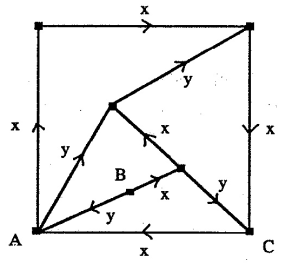
\includegraphics[width=5cm]{Images/diagrama_quaternios.png}
			\end{center}
		\caption{Diagrama de van Kampen para o grupo dos quatérnios, $Q_8$}
		\label{figura diagrama quaternios}
		\end{figure}
	\par\vspace{0.3cm} Na parte superior da face esquerda, a fronteira, lida no sentido horário a partir de $A$ é $s = x^2y^{-2}$. De modo análogo, a face contendo $B$, lida no sentido anti-horário a partir de $B$ também nos dá $s = x^2y^{-2}$. Na face inferior contendo $B$, a delimitação do bordo lida no sentido horário a partir de $A$ nos dá $t = y^{-1}xyx$. Do mesmo modo, a face mais à direita, lida no sentido horário a partir de $C$ também nos dá $t = y^{-1}xyx$. Por fim, como a marca sobre a fronteira, lida no sentido horário a partir de $A$, é $x^4=1$, isso nos mostra que essa primeira relação na apresentação de $Q_8$ é supérflua.	
	\par\vspace{0.3cm} Outro exemplo é o grupo 
		\begin{equation*}
		G = \langle a,b,c,d \ | \ ab = c, bc = d, cd = a, da = b \rangle
		\end{equation*}
		\par\vspace{0.3cm} é claramente gerado por $a$ e $b$, uma vez que $c = ab$ e $d = bc = bab$. Contudo, esse fato pode ser verificado a partir do diagrama de van Kampen para essa apresentação. Nele, as faces estão marcadas pelas seguintes relações definidoras:
		\begin{equation*}
		r_1 = abc^{-1}, \ r_2 = bcd^{-1}, \ r_3 = cda^{-1}, \ r_4 = dab^{-1}
		\end{equation*}
		\begin{figure}[H]
			\begin{center}
				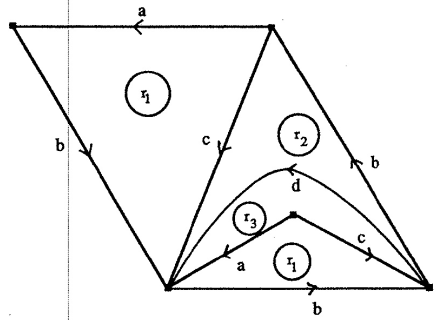
\includegraphics[width=7.5cm]{Images/diagrama_ciclico.png}
			\end{center}
		\caption{Diagrama de van Kampen de $G$}
		\label{figura diagrama ciclico}
		\end{figure}
		\par\vspace{0.3cm} A partir do diagrama, vemos que lendo a fronteira, no sentido anti-horário, a partir do vértice superior direito, temos $ab^3 = 1$, ou seja, $a = b^{-3}$ e, portanto, $G$ é gerado apenas por $b$, sendo cíclico. De fato, podemos fazer uma manipulação desse diagrama para obter o seguinte diagrama:
		\begin{figure}[H]
			\begin{center}
				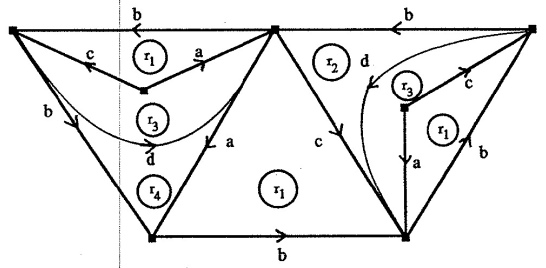
\includegraphics[width=7.5cm]{Images/diagrama_ciclico_2.png}
			\end{center}
		\caption{Diagrama de van Kampen manipulado de $G$}
		\label{figura diagrama ciclico 2}
		\end{figure}
	\par\vspace{0.3cm} A partir desse diagrama, vemos, a partir da leitura do bordo, que $b^5=1$. Logo, $G$ é o grupo cíclico de ordem $5$ ($b$ não trivial) ou $1$ ($b$ trivial).
	\par\vspace{0.3cm} É interessante notar que se $a$, $b$, $c$ e $d$ são geradores de um grupo tais que $a$ e $b$ comutam com $c$ e $d$, então o fato de que $ab$ comuta com $cd$ pode ser deduzido pelo seguinte diagrama:
		\begin{figure}[H]
			\begin{center}
				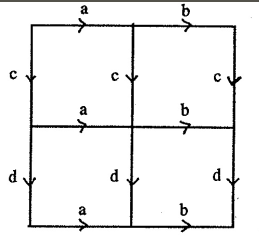
\includegraphics[width=5cm]{Images/diagrama_comutatividade.png}
			\end{center}
		\caption{Diagrama de van Kampen em que $a$ e $b$ comutam com $c$ e $d$}
		\label{figura diagrama comutatividade}
		\end{figure}
	\par\vspace{0.3cm} Do diagrama, é imediato que $abcd(ab)^{-1}(cd)^{-1} = 1$, ou seja, $[ab,cd] = 1$.	
	\par\vspace{0.3cm} Um último exemplo é o seguinte: fazendo $r = x^2yxy^3 = 1 = y^2xyx^3 = s$, obtemos o seguinte diagrama:
		\begin{figure}[H]
			\begin{center}
				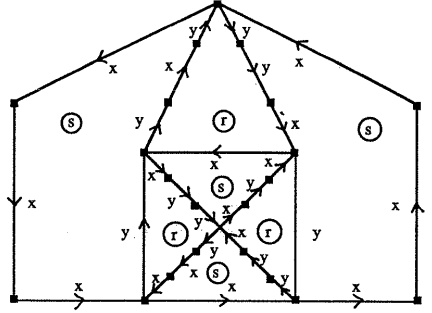
\includegraphics[width=7.5cm]{Images/diagrama_complicado.png}
			\end{center}
		\end{figure}
		\par\vspace{0.3cm} Da leitura do bordo no sentido anti-horário, obtemos $x^7=1$.
	\par\vspace{0.3cm} Dos exemplos acima, podemos ver que os diagramas de van Kampen nos ajudam a deduzir relações que não são tão imediatas tendo apenas a apresentação do grupo.
	
	\section{Tranças como discos perfurados}\label{secao trancas como discos perfurados}
	\hspace{12pt} Podemos, ainda, pensar em tranças de uma terceira maneira. Voltando na trança da Figura \eqref{tranca espaco configuracao}, vamos imaginar o seguinte: suponha que a trança é feita de fios rígidos, e que o plano é, na verdade, uma seção quadrada do plano (como está desenhado), ou seja, um disco topológico, exceto que esse disco tem buracos.
	\par\vspace{0.3cm} Agora, imagine que o interior do disco é feito de um material muito flexível e que a fronteira (bordo) quadrada é uma armação rígida (parecida com aqueles \textit{frisbees} de tecido, apenas quadrados). Imagine o processo de empurrar esse disco perfurado ao longo da trança de fios rígidos até chegar na parede da direita. A trança não se moveu, mas o disco em si foi todo torcido, ou seja, a trança provocou uma mudança na superfície.
	\par\vspace{0.3cm} Mais especificamente, o que aconteceu ao disco perfurado foi que a trança implementou um homeomorfismo da superfície nela mesma. O bordo fica fixo, porque é rígido, e as perfurações são permutadas conforme a permutação associada à trança. Funções como essa, a menos de homotopia, formam o \textit{grupo de classes} de $D_n$, um disco com $n$ perfurações com bordo $\partial D_n$ (e não o grupo diedral):
	\begin{align*}
	\Mod(D_n) = \{ f:D_n\to D_n|& f\text{ é homeomorfismo}, \\
	&f|_{\partial D_n} = 1 \}/\text{Homotopia}
	\end{align*}
	
	\begin{figure}[H]
		\begin{center}
			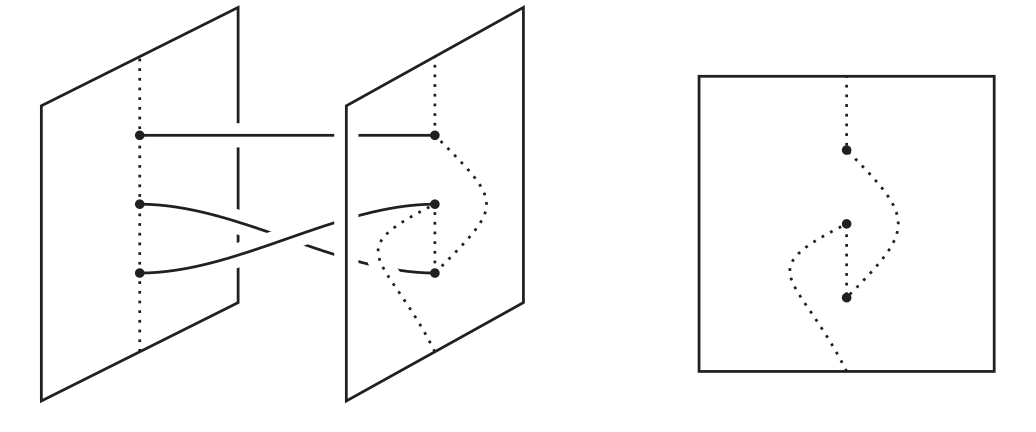
\includegraphics[width=10cm]{Images/tranca_disco_perfurado.png}
		\end{center}\caption{Diagrama de curva associado a $\sigma_1$.}
		\label{tranca disco perfurado}
	\end{figure}
	
	\par\vspace{0.3cm} A operação do grupo é a composição de funções: dois homeomorfismos $f$ e $g$ podem ser compostos para formar um homeomorfismo $g\circ f$ (ou $f\circ g$, que geralmente é diferente). Acima, descrevemos uma função $\psi: B_n\to\Mod(D_n)$, a saber, dada uma trança, deslize o disco pela trança e considere o homeomorfismo resultante. De fato, $\psi$ é, na verdade, um isomorfismo.
	
	\begin{theorem}
		\label{B_n isomorfo a Mod(D_n)}
		$B_n\cong \Mod(D_n)$ 
	\end{theorem}
	
	\begin{proof}
		Não demonstraremos a sobrejetividade de $\psi$, pois exige conhecimentos além do escopo deste relatório.
		\par\vspace{0.3cm} Primeiro, note que $\psi$ está bem definida, pois se $\alpha, \beta\in B_n$ são tais que $\alpha = \beta$, então elas induzem a mesma deformação no disco, i.e., o mesmo homeomorfismo e, portanto, temos $\psi(\alpha) = \psi(\beta)$.
		\par\vspace{0.3cm} Além disso, o núcleo de $\psi$ é, por definição, formado pelas tranças que induzem o homeomorfismo identidade, ou seja, as tranças que não fazem nada com o interior do disco (o bordo fica fixo sempre). Ora, mas a única trança que não deforma o interior do disco é a identidade e, portanto, $\Ker\psi = \{1\}$.
		\par\vspace{0.3cm} Agora, sejam $\alpha, \beta\in B_n$ duas tranças quaisquer tais que $\psi(\alpha) = f$ e $\psi(\beta) = g$. Daí, temos
		\begin{align*}
		\psi(\alpha\beta) = g\circ f = \psi(\alpha)\circ\psi(\beta)
		\end{align*}
		\par\vspace{0.3cm} Essa última igualdade nos diz simplesmente que, fazendo o produto de duas tranças $\alpha$ e $\beta$, a deformação resultante é equivalente a aplicar a deformação da segunda trança ($\beta$) na deformação da primeira trança ($\alpha$), ou seja, compor as duas deformações. 
		\par\vspace{0.3cm} Portanto, como $\psi$ é um homomorfismo sobrejetor de núcleo trivial, então $B_n\cong\Mod(D_n)$.
	\end{proof}
	
	\subsection{Diagramas de curvas}
	\hspace{12pt} Vamos nos aprofundar um pouco nessa nova perspectiva dos grupos de tranças. Olhe novamente a Figura \eqref{tranca espaco configuracao}, mas foque agora nos discos quadrados perfurados nas extremidades da imagem. Imagine que há uma linha vertical pontilhada no disco da esquerda passando por todas as perfurações. A pergunta é: para onde irá a linha pontilhada após deslizarmos o disco pela trança?
	\par\vspace{0.3cm} A Figura \eqref{tranca disco perfurado} mostra um exemplo mais simples. Nela, a trança é simplesmente $\sigma_1$, e tanto a linha pontilhada original quanto o resultado torcido estão desenhados. A linha pontilhada na parede da direita é dita \textit{diagrama de curva} induzido pela trança ($\sigma_1$, nesse caso). 
	\par\vspace{0.3cm} Vamos chamar a linha pontilhada original de \textbf{eixo} do disco. Ele consiste de $n+1$ segmentos pontilhados $a_0, \dots, a_n$, numerados em ordem de baixo para cima. Então, em geral, o diagrama de curva associado a uma trança $\beta$ é a união dos arcos $\psi_{\beta}(a_i)$ (os arcos que são as imagens dos $a_i$'s), i.e., você pensa em $\beta$ como um homeomorfismo do disco e o diagrama de curva é para onde o eixo vai (a imagem do eixo). 
	\par\vspace{0.3cm} Denotaremos os arcos do diagrama de curva por $c_i$, e o diagrama todo por $c$. Note que, como $\beta$ fixa $\partial D_n$ (o bordo), os $c_i$'s (isto é, o diagrama de curva) se encaixam ponta a ponta, em ordem, para formar o único arco $c$ que começa no centro inferior, nunca se cruza, passa por cada perfuração uma única vez e termina no centro superior. Veja novamente a Figura \eqref{tranca disco perfurado}.  
	\par\vspace{0.3cm} Diagramas de curva podem ser extremamente complicados, como poderíamos esperar se tivermos uma trança longa. Por exemplo, o diagrama de curva da trança da Figura \eqref{tranca espaco configuracao} é bem complicado de desenhar. 
	\par\vspace{0.3cm} Uma maneira preliminar de simplificar um diagrama de curva é ter certeza de que ele está \textit{reduzido}, no seguinte sentido: dado um diagrama de cruva em um disco perfurado, desenhe o eixo no mesmo disco. O diagrama é dito \textit{reduzido} se não existem \textit{biágonos} na figura, i.e., regiões cujas fronteiras consistem de um subarco de um único $a_i$ e um subarco de um único $c_i$. 
	\par\vspace{0.3cm} Podemos resumir o que foi dito no parágrafo anterior nas seguintes definições:
	\begin{deff}
		\label{def biagono}
		Um biágono é um região cuja fronteira consiste de um subarco de um único $a_i$ e um subarco de um único $c_i$.
	\end{deff}
	\begin{deff}
		\label{def reducao}
		Um diagrama de curva é dito reduzido quando não possui biágonos.
	\end{deff}
	\par\vspace{0.3cm} Os biágonos podem ser facilmente eliminados, de modo que todo diagrama de curva pode ser reduzido. 
	
	\begin{figure}[H]
		\begin{center}
			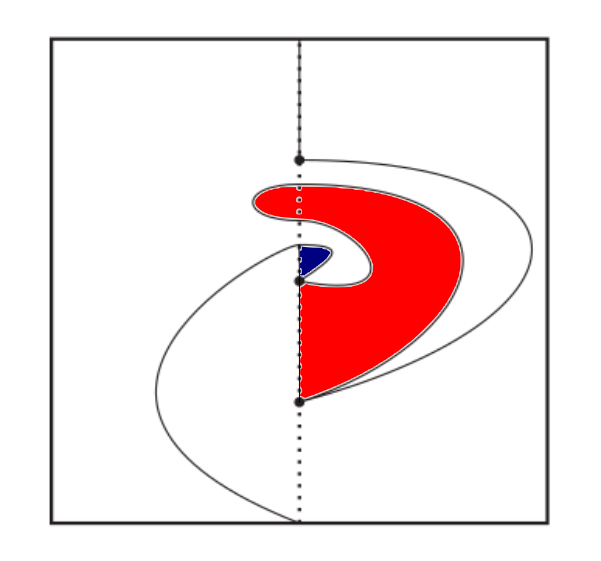
\includegraphics[width=7cm]{Images/biagonos.png}
		\end{center}\caption{Esse diagrama possui 2 biágonos (em vermelho e em azul), e pode ser reduzido ao diagrama da Figura \eqref{tranca disco perfurado}.}
		\label{diagrama nao reduzido com biagonos}
	\end{figure}
	\par\vspace{0.3cm} É, então, natural considerar os diagramas das Figuras \eqref{tranca disco perfurado} e \eqref{diagrama nao reduzido com biagonos} como equivalentes. Esse fato nos leva à seguinte definição.
	
	\begin{deff}
		\label{def equivalencia diagramas}
		Dois diagramas de curva são ditos equivalentes se têm a mesma forma reduzida.
	\end{deff}  
	\par\vspace{0.3cm} Vamos, agora, mostrar uma aplicação interessante dos diagramas de curva, a saber, na demonstração da Proposição \eqref{geradores de B_n tem ordem infinita}.
	\par\vspace{0.3cm} Dada uma trança $\beta$, vamos olhar para o seu diagrama de curva $c$. Começe na parte de baixo e observe o primeiro arco $c_i$ que não é igual ao arco correspondente $a_i$ no eixo. Se $c_i$ está à direita de $a_i$, dizemos que $\beta$ é \textit{desviada à direita} e, se $c_i$ está à esquerda de $a_i$, dizemos que $\beta$ é \textit{desviada à esquerda}. Se $c_i = a_i$ para todo $i$, então $\beta$ é a trança identidade (tecnicamente, estamos usando o Teorema \eqref{B_n isomorfo a Mod(D_n)}). A trança da Figura \eqref{tranca disco perfurado} é desviada à esquerda, pois começando na parte inferior, o arco $c_0$ desvia para a esquerda.
	\begin{prop}
		\label{desvio a direita desvio a esquerda}
		Se $\beta$ é desviada à esquerda, então $\beta^{-1}$ é desviada à direita.
	\end{prop}
	\begin{proof}
		O efeito, no diagrama de curva, de inverter uma trança é simplesmente realizar uma reflexão em torno de uma das arestas do disco paralelas ao eixo. Observe a Figura \eqref{diagrama inverso de sigma1}.
		\begin{figure}[H]
			\begin{center}
				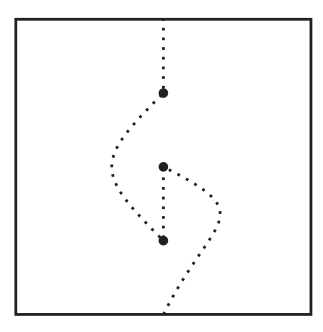
\includegraphics[width=5cm]{Images/inverso.png}
			\end{center}\caption{Diagrama de curva de $\sigma_1^{-1}$}\label{diagrama inverso de sigma1}
		\end{figure}
		\par\vspace{0.3cm} Portanto, como inverter uma trança equivale a refletir o seu diagrama de curva, segue que se a trança original era desviada à esquerda, o seu inverso será desviado à direita e vice-versa.
	\end{proof}
	\par\vspace{0.3cm} Queremos mostrar que $B_n$ é livre de torção. Esse fato segue do seguinte lema.
	
	\begin{lemma}
		\label{desviada a direita, sempre a direita}
		Se $\beta$ é desviada à direita, então $\beta^n$ é desviada à direita para todo $n>0$.
	\end{lemma}
	\begin{proof}
		Suponha que $\beta$ é desviada à direita, e observe o diagrama de curva reduzido $c$ de $\beta$. Encontre o primeiro $c_i$ que difere do $a_i$ correspondente, e chame esse arco de $c_k$. Denotando por $c^2$ o diagrama de curva de $\beta^2$, e por $c_i^2$ os arcos de $c^2$, imagine dois discos separados: um em que $a_i$ e $c_i$ estão desenhados e um em que $c_i$ e $c_i^2$ estão desenhados. Observe que a segunda figura é obtida da primeira aplicando a trança $\beta$ (pensada como um homeomorfismo). Então, como $c_k$ está à direita de $a_k$, segue que $c_k^2$ está à direita de $c_k$. Além disso, como não há biágonos na primeira figura, também não há biágonos na segunda figura.
		\par\vspace{0.3cm} Queremos mostrar que $\beta^2$ é desviada à direita, i.e, que $c_k^2$ está à direita de $a_k$. Sabemos que $\beta$ não afeta os arcos $a_i$ para $i<k$, e então $\beta^2$ também não. Também sabemos que, nas figuras, $c_k$ está à direita de $a_k$ e $c_k^2$ está à direita de $c_k$.
		\par\vspace{0.3cm} O que falta observar é que o diagrama de $\beta^2$ pode não estar reduzido. Sabemos que não há biágonos entre o eixo e $c$, e também que não há biágonos entre $c$ e $c^2$, mas se $c^2$ e o eixo formarem um biágono, então $c^2$ precisa ser reduzido e pode acabar não sendo desviado à direita.
		\par\vspace{0.3cm} Felizmente, isso não ocorre. Para ver que esse é o caso, seja $d$ o segmento inicial de $c_k$ que vai até a primeira vez que $c_k$ intercepta o eixo, de forma que $d$ está contido em uma metade (a metade da direita) do disco (é possível que $d$ seja $c_k$ inteiro, mas em geral $c_k$ pode ``passear'' bastante antes de atingir uma perfuração). Agora, a única maneira de $c_k^2$ estar à esquerda (ou ser igual) do arco $a_k$ do eixo é formando um biágono com $a_k$. Mas isso forçaria $c_k^2$ a cruzar $d$, criando um biágono entre $c$ e $c^2$, o que sabemos que não existe. Veja a figura abaixo.
		
		\begin{figure}[H]
			\begin{center}
				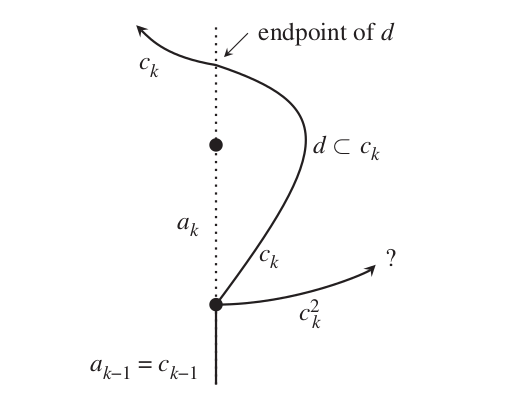
\includegraphics[width=8cm]{Images/demosntracao_lema.png}
			\end{center}\caption{Ilustração da demonstração}
			\label{ilustracao da demonstracao}
		\end{figure}
		\par\vspace{0.3cm} Portanto, $\beta^2$ é, de fato, desviada à direita. Repetindo o argumento, mostramos que $\beta^n$ é desviada à direita para todo $n>0$.
	\end{proof}
	
	\begin{corollary}
		\label{B_n livre de torcao por diagramas de curva}
		$B_n$ é livre de torção.
	\end{corollary}
	\begin{proof}
		Do Lema \eqref{desviada a direita, sempre a direita}, sabemos que se $\beta$ é desviada à direita, $\beta^n$ também o é para todo $n$ positivo. Da Proposição \eqref{desvio a direita desvio a esquerda}, sabemos que $\beta^{-1}$ é desviada à esquerda e então, novamente do Lema \eqref{desviada a direita, sempre a direita}, $(\beta^{-1})^n$ também o é para todo $n$ positivo. Portanto, toda trança que é desviada (seja à direita ou à esquerda) tem ordem infinita. Como, do Teorema \eqref{B_n isomorfo a Mod(D_n)}, a trança trivial é a única trança que não é desviada, temos que $B_n$ é livre de torção.
	\end{proof}
	
	\begin{remark}
		Na demonstração do Lema \eqref{desviada a direita, sempre a direita}, alguns detalhes foram omitidos. Por exemplo, homeomorfismos podem ser complicados: poderia ser o caso de que o arco $c_0$ interceptasse $a_0$ infinitas vezes. Então, como reduzi-lo? Esse e outros detalhes podem ser tratados de maneira rigorosa, o que está além do escopo desse relatório.
	\end{remark}
	
	\par\vspace{0.3cm} Uma última aplicação interessante dessa nova visualização dos grupos de trança é na identificação de tranças (palavras) que são equivalentes à identidade, ou seja, o problema da palavra (veja Seção \ref{secao o problema da palavra}). Usando o Teorema \eqref{B_n isomorfo a Mod(D_n)}, sabemos que uma trança $\beta$ é trivial se, e só se, $\psi(\beta) = \text{Id}$, ou seja, se, e só se, $\beta$ induz o homeomorfismo identidade (não faz nada com o disco). Portanto, dada uma trança $\beta$ qualquer, basta observarmos o efeito de $\beta$ no disco perfurado: se provoca torção, não é trivial; se não provoca torção, é trivial. Esse procedimento é complicado de computar para tranças longas, mas continua sendo uma solução igualmente válida.